% ========================================
% DOCUMENTO PRINCIPAL - VALUACIÓN DE EMPRESAS TECNOLÓGICAS
% ========================================

\documentclass[12pt,a4paper,twoside]{report}

% ========================================
% PAQUETES Y CONFIGURACIÓN
% ========================================
\usepackage[utf8]{inputenc}
\usepackage[spanish,es-tabla]{babel}
\usepackage[T1]{fontenc}
\usepackage{lmodern}

% Geometría y márgenes profesionales
\usepackage{geometry}
\geometry{
    left=2.5cm,
    right=2.5cm,
    top=2.5cm,
    bottom=2.5cm
}

% Matemáticas y símbolos
\usepackage{amsmath,amssymb,amsfonts}
\usepackage{mathtools}

% Gráficos y figuras
\usepackage{graphicx}
\usepackage{float}
\usepackage[font=small,labelfont=bf]{caption}
\usepackage{subcaption}

% Tablas avanzadas
\usepackage{booktabs}
\usepackage{array}
\usepackage{multirow}
\usepackage{longtable}

% Colores y enlaces
\usepackage{xcolor}
\usepackage[hidelinks]{hyperref}
\usepackage{url}

% Comillas y bibliografía con estilo APA
\usepackage{csquotes}
\usepackage[style=apa,backend=biber,natbib=true]{biblatex}
\addbibresource{referencias.bib}

% Espaciado y formato
\usepackage{setspace}
\onehalfspacing
\usepackage{indentfirst}
\setlength{\parindent}{1.25cm}

% Encabezados y pies de página
\usepackage{fancyhdr}
\pagestyle{fancy}
\fancyhf{}
\fancyhead[R]{\thepage}
\fancyhead[L]{\leftmark}
\renewcommand{\headrulewidth}{0.4pt}

% Numeración de secciones
\setcounter{secnumdepth}{3}
\setcounter{tocdepth}{3}

% Personalización de capítulos
\usepackage{titlesec}
\titleformat{\chapter}[display]
{\normalfont\huge\bfseries}{\chaptertitlename\ \thechapter}{20pt}{\Huge}

% ========================================
% INFORMACIÓN DEL DOCUMENTO
% ========================================
\title{Valuación de empresas tecnológicas: Fundamentos, métodos y tendencias actuales}
\author{[Su Nombre]}
\date{\today}

% ========================================
% INICIO DEL DOCUMENTO
% ========================================
\begin{document}

% Portada
\begin{titlepage}
    \centering
    
    % Logo de la universidad (si lo tienes)
    % \includegraphics[width=0.3\textwidth]{figuras/logo_universidad.png}\\[1cm]
    
    {\Large \textbf{UNIVERSIDAD DE BUENOS AIRES}}\\[0.5cm]
    {\large Facultad de Ciencias Económicas}\\[0.5cm]
    {\large Departamento de Finanzas}\\[2cm]
    
    {\huge \textbf{Valuación de empresas tecnológicas}}\\[0.5cm]
    {\Large \textbf{Fundamentos, métodos y tendencias actuales}}\\[2cm]
    
    {\large Trabajo Final de Grado}\\[0.5cm]
    {\large Materia: Valuación de Activos}\\[3cm]
    
    \begin{minipage}{0.4\textwidth}
        \begin{flushleft} \large
            \emph{Autor:}\\
            {[Su Nombre Completo]}\\
            {[Número de Legajo]}
        \end{flushleft}
    \end{minipage}
    \begin{minipage}{0.4\textwidth}
        \begin{flushright} \large
            \emph{Profesor:}\\
            {[Nombre del Profesor]}
        \end{flushright}
    \end{minipage}\\[3cm]
    
    {\large Buenos Aires, Argentina}\\[0.5cm]
    {\large \today}
    
    \vfill
\end{titlepage}

\cleardoublepage 

% Índice
\cleardoublepage
\tableofcontents
\cleardoublepage

% Contenido principal
\chapter{Introducción}

En las últimas décadas, las empresas del sector tecnológico han pasado a dominar los mercados bursátiles globales. Compañías como Apple, Amazon, Google, Meta o Microsoft se encuentran entre las de mayor capitalización del mundo, reflejando el auge de la economía digital y basada en activos intangibles. En 2024, los activos intangibles corporativos globales alcanzaron aproximadamente 80 billones de dólares, representando el 90\% del valor del S\&P 500 \citep{wipo2025,oceantomo2024}. La valuación de empresas tecnológicas se ha convertido así en un tema crucial tanto para inversores como para académicos, especialmente desde episodios históricos como la burbuja \emph{puntocom} de finales de los años 90 hasta las valoraciones récord de \emph{startups} unicornio en tiempos recientes.

La evolución del sector tecnológico ha experimentado un cambio paradigmático significativo en 2024, marcado por el auge de la Inteligencia Artificial que ha recibido el 48\% de toda la inversión de capital de riesgo global, superando los 100 mil millones de dólares en financiamiento ---un incremento del 80\% interanual--- \citep{pitchbook2024}. Este fenómeno ha redefinido los criterios de valuación, donde las empresas tecnológicas deben ahora demostrar no solo innovación, sino también un camino claro hacia la rentabilidad, con requisitos de ingresos para financiamiento Serie A que han aumentado 75\% desde 2021, alcanzando una mediana de 2.5 millones de dólares \citep{carta2024}.

Valuar una empresa consiste esencialmente en estimar su valor económico, lo cual sirve para fundamentar decisiones de inversión, procesos de adquisición o fusiones, salidas a bolsa y estrategias corporativas. En el caso de las firmas tecnológicas, este ejercicio presenta desafíos particulares: a menudo operan con modelos de negocio innovadores, crecimiento acelerado, ingresos difíciles de predecir y activos intangibles (como \emph{software}, datos, patentes o marca) que no siempre aparecen reflejados en sus balances financieros tradicionales.

Además, muchas \emph{startups} tecnológicas muestran pérdidas en sus primeros años mientras construyen una base de usuarios o desarrollan productos disruptivos. La realidad actual del mercado refleja esta complejidad: aproximadamente el 50\% de las empresas unicornio ---aquellas valuadas en más de mil millones de dólares--- posiblemente ya no merecen ese estatus según criterios de mercado justo, con el 30\% de ellas actualmente valuadas por debajo del umbral de mil millones según valoraciones ajustadas al mercado \citep{silicon2024}. Todos estos factores hacen que los métodos clásicos de valoración deban adaptarse o complementarse para capturar adecuadamente el valor real de estas compañías.

\section{Objetivos}

El objetivo general de esta investigación es analizar los fundamentos teóricos y metodológicos de la valuación de empresas tecnológicas, identificando las particularidades que distinguen este sector y las tendencias actuales en criterios de valoración en la era digital.

Para alcanzar este propósito principal, se examina el marco teórico general de valoración empresarial y su aplicación específica al sector tecnológico, se identifican y analizan los métodos más utilizados en la valuación de estas empresas, y se caracterizan las particularidades que afectan su valoración. Asimismo, se evalúan los factores cuantitativos y cualitativos que inciden en la valoración de empresas \emph{tech}, se analizan casos de estudio representativos del sector, y se identifican las tendencias actuales que están moldeando los criterios de valoración en el contexto de la transformación digital.

\section{Justificación}

La creciente importancia de las empresas tecnológicas en la economía global y su peso en los mercados financieros hace necesario comprender profundamente los métodos y criterios utilizados para su valoración. Este trabajo contribuye al conocimiento académico y profesional en un área donde los métodos tradicionales de valoración enfrentan desafíos significativos debido a las características particulares del sector tecnológico.

\section{Metodología}

Este trabajo de investigación se basa en una revisión exhaustiva de literatura académica y profesional, análisis de casos de estudio representativos y examen de tendencias actuales en el mercado. Se utiliza un enfoque descriptivo-analítico que combina el marco teórico de valoración financiera con las particularidades del sector tecnológico.

\section{Estructura del trabajo}

En este trabajo de investigación se exploran los fundamentos teóricos de la valuación de empresas, los métodos más utilizados aplicados al sector tecnológico, las características específicas de las empresas tech que afectan su valuación, los factores cuantitativos y cualitativos que inciden en su valor, casos de estudio representativos y las tendencias actuales en criterios de valuación en la era digital.

La estructura sigue un formato académico: primero se presenta el marco teórico general de valoración, luego el desarrollo con el análisis específico del ámbito tecnológico ---incluyendo métodos, factores y casos prácticos---, para finalmente exponer las conclusiones principales y la bibliografía empleada. 
\chapter{Marco Teórico}

La teoría financiera establece que el valor de una empresa se basa en la capacidad de ésta para generar flujos de fondos futuros y en el riesgo asociado a dichos flujos. En términos generales, \textbf{el valor intrínseco de una empresa en marcha es el valor presente de sus flujos de caja futuros esperados, descontados a una tasa que refleje el riesgo de la empresa}.

Este enfoque de \emph{descuento de flujos} considera a la empresa como un ente generador de caja, cuyo patrimonio (acciones) y deuda pueden valorarse al igual que otros activos financieros en función de esos flujos.

\section{Método de Flujo de Caja Descontado (DCF)}

Para aplicar esta metodología, comúnmente denominada \textbf{Flujo de Caja Descontado} (\emph{DCF, Discounted Cash Flow}), es necesario proyectar los flujos de caja libres futuros de la empresa y determinar una tasa de descuento apropiada. Por lo general, se utiliza el costo promedio ponderado de capital o \emph{WACC}, que combina el costo de la deuda y del capital propio.

El resultado es una estimación del valor presente neto de la empresa, considerando su continuidad operacional indefinida. Los métodos basados en DCF son considerados conceptualmente los más correctos para valorar empresas en marcha con perspectivas de continuidad, ya que se fundamentan en principios financieros sólidos (valor tiempo del dinero, relación riesgo-retorno, etc.) \citep{copeland2014,damodaran2012}.

\section{Enfoques principales de valuación}

En la práctica existen diversos enfoques y métodos de valuación que pueden agruparse en tres categorías principales, cada una con sus fundamentos teóricos específicos y aplicaciones apropiadas según el contexto empresarial.

\subsection{Enfoque de ingresos y valor intrínseco}

El enfoque de ingresos incluye el método de descuento de flujos de caja (\emph{DCF}) y sus variantes como el descuento de dividendos o el modelo de valor presente ajustado. Todos ellos comparten la lógica fundamental de calcular el valor presente de beneficios futuros esperados, constituyendo el marco teórico más sólido para la estimación del valor intrínseco empresarial. Este enfoque reconoce que el valor de una empresa deriva de su capacidad de generar flujos de caja libres a sus inversionistas, descontados a una tasa que refleje apropiadamente el riesgo asociado a dichos flujos.

También en esta categoría se inscribe el concepto de \textbf{Valor Económico Agregado} (\emph{EVA}), que mide la utilidad económica residual de la empresa calculada como el beneficio operativo neto menos el costo de oportunidad del capital total invertido. La capitalización a perpetuidad del \emph{EVA} puede utilizarse como método alternativo para valorar la empresa, proporcionando una perspectiva complementaria que enfatiza la creación de valor por encima del costo de capital. Este enfoque resulta particularmente útil para evaluar el desempeño gerencial y la eficiencia en el uso de recursos, aunque presenta limitaciones similares al \emph{DCF} en términos de dependencia de proyecciones futuras.

El método de descuento de flujos constituye el pilar central de la teoría de valuación financiera debido a su fundamentación en principios económicos establecidos. Su fortaleza radica en la consideración explícita del valor tiempo del dinero, la incorporación del riesgo a través de la tasa de descuento, y su capacidad para reflejar las características específicas del negocio mediante las proyecciones de flujos de caja. Sin embargo, su aplicación práctica enfrenta desafíos significativos relacionados con la sensibilidad a supuestos sobre crecimiento futuro, márgenes operativos, inversiones requeridas, y la determinación apropiada de la tasa de descuento.

En empresas tecnológicas, estos desafíos se magnifican debido a la mayor incertidumbre inherente en sus proyecciones financieras, la dificultad de estimar flujos de caja en negocios con modelos emergentes, y la necesidad de capturar el valor de opciones de crecimiento futuro que pueden representar una porción significativa del valor total. Por tanto, aunque el \emph{DCF} mantiene su posición como método de referencia, su aplicación en el contexto tecnológico requiere adaptaciones metodológicas específicas y frecuentemente debe complementarse con enfoques alternativos.

\subsection{Enfoque de mercado y valuación relativa}

El enfoque de mercado comprende los métodos de múltiplos comparables, que valoran la empresa en relación con otras similares mediante la aplicación de indicadores financieros representativos. Los múltiplos más utilizados incluyen \textbf{Precio/Beneficio} (\emph{P/E}), \textbf{Valor Empresa/\emph{EBITDA}}, \textbf{Valor Empresa/Ventas}, y otros específicos del sector. La lógica subyacente consiste en estimar el valor implícito de la empresa si el mercado la valorase de forma análoga a sus pares comparables, asumiendo que empresas similares en términos de riesgo, crecimiento, y rentabilidad deberían comercializarse a múltiplos similares.

Los métodos de múltiplos gozan de gran popularidad en la práctica profesional debido a su simplicidad de aplicación, su capacidad para reflejar las condiciones actuales del mercado, y su utilidad para proporcionar rangos de valoración que pueden contrastarse con resultados obtenidos mediante otros métodos. Además, estos métodos incorporan implícitamente las expectativas y percepciones agregadas del mercado sobre las perspectivas futuras del sector, lo cual puede resultar valioso para capturar tendencias y sentimientos que podrían no estar completamente reflejados en análisis fundamentales individuales.

No obstante, desde una perspectiva teórica estricta, los múltiplos se consideran aproximaciones que deben emplearse con cautela y preferiblemente como complemento del valor obtenido por descuento de flujos. Como señala \cite{fernandez2007}, los múltiplos per se constituyen métodos conceptualmente limitados que asumen eficiencia de mercado y comparabilidad perfecta entre empresas, supuestos que frecuentemente no se cumplen en la realidad. La identificación de empresas verdaderamente comparables representa un desafío particular, especialmente en sectores dinámicos como la tecnología donde las diferencias en modelos de negocio, etapa de desarrollo, y exposición geográfica pueden ser significativas.

En el contexto de empresas tecnológicas, el enfoque de múltiplos presenta ventajas y limitaciones específicas. Por una parte, permite capturar rápidamente el sentimiento del mercado hacia empresas del sector y proporciona referencias útiles para valoraciones en mercados privados donde las transacciones comparables pueden ser escasas. Por otra parte, la volatilidad inherente de los múltiplos tecnológicos, la dificultad de encontrar comparables apropiados para modelos de negocio innovadores, y la tendencia del mercado a valorar expectativas especulativas pueden generar distorsiones significativas en las estimaciones de valor.

\subsection{Métodos especializados y enfoques híbridos}

Además de los enfoques tradicionales, existen métodos especializados particularmente relevantes para la valoración de empresas tecnológicas, incluyendo el enfoque de activos, el método de opciones reales, y técnicas específicas del capital de riesgo. El enfoque de activos considera el valor de los activos netos de la empresa, ya sea en marcha o en caso de liquidación, mediante la evaluación del valor en libros ajustado o el valor de liquidación. Para empresas tecnológicas en crecimiento, este enfoque suele ser menos relevante puesto que el valor de sus activos intangibles fundamentales ---algoritmos, bases de datos, capital humano, relaciones con clientes--- no aparece completamente reflejado en el balance general. Sin embargo, puede proporcionar un piso de valor en casos de empresas maduras o en dificultades financieras.

El método de opciones reales constituye una aplicación de la teoría de opciones financieras a la valoración de empresas o proyectos, reconociendo explícitamente la flexibilidad gerencial y las oportunidades de crecimiento como opciones valiosas. Este método resulta particularmente apropiado para empresas tecnológicas que poseen opciones de expandir proyectos exitosos, entrar en nuevos mercados geográficos o de productos, posponer inversiones hasta obtener información adicional, o abandonar proyectos que no cumplan expectativas. Valorar estas opciones de crecimiento puede revelar valor oculto en empresas con alto potencial pero flujos de caja actuales bajos o negativos, situación común en \emph{startups} tecnológicas.

La aplicación práctica del método de opciones reales enfrenta desafíos técnicos relacionados con la estimación de volatilidades apropiadas, la identificación y valoración de opciones específicas, y la determinación de parámetros del modelo. Sin embargo, proporciona un marco conceptual valioso para comprender por qué el mercado puede asignar valoraciones aparentemente excesivas a empresas tecnológicas jóvenes: gran parte del valor puede residir en opciones futuras más que en flujos de caja inmediatos.

El método \emph{Venture Capital} utilizado por inversores de capital de riesgo para \emph{startups} consiste en estimar un valor futuro de salida ---venta estratégica o salida a bolsa--- y descontarlo a una tasa de retorno objetivo elevada que refleje el riesgo extraordinario, frecuentemente entre 30\% y 50\% anual en etapas tempranas. Es básicamente una variante del \emph{DCF} enfocada en el valor terminal con un horizonte de salida específico, combinada con consideraciones sobre la dilución esperada por futuras rondas de inversión y la probabilidad de éxito o fracaso total.

En resumen, el marco teórico de valuación provee múltiples enfoques complementarios, donde el método de flujo de caja descontado permanece como el pilar central y conceptualmente más sólido para valorar empresas. En la práctica profesional, estos métodos se combinan frecuentemente para proporcionar rangos de valoración que incorporen diferentes perspectivas sobre el valor empresarial. El análisis que sigue en el desarrollo profundiza cómo se aplican y adaptan estos métodos al caso particular de las empresas tecnológicas, y qué características distintivas de estas compañías inciden en los resultados de valuación. 
\chapter{Desarrollo}

En este capítulo se analiza específicamente la aplicación de los fundamentos teóricos de valuación al sector tecnológico, explorando los métodos más utilizados, las características particulares de estas empresas, los factores que inciden en su valoración, casos representativos y las tendencias actuales.

% Incluir las subsecciones modulares
\section{Métodos más utilizados en la valuación de empresas tecnológicas}

En el ámbito tecnológico se emplean los mismos métodos generales descritos en el marco teórico, aunque con matices importantes. A continuación, se resumen los métodos más relevantes, destacando su uso y desafíos al aplicarlos a empresas tecnológicas.

\subsection{Flujo de Caja Descontado}

El método de \emph{DCF} sigue siendo la herramienta de referencia para valorar empresas \emph{tech} maduras o con proyecciones financieras estructuradas \citep{kruze2023}, aunque presenta desafíos particulares en el contexto tecnológico. En emprendimientos emergentes, los flujos de caja suelen ser negativos en los primeros años y altamente inciertos, lo que complica significativamente la estimación del valor intrínseco.

La aplicación práctica del \emph{DCF} en empresas tecnológicas requiere modelos de etapas múltiples que proyectan un periodo inicial de crecimiento alto ---frecuentemente acompañado de pérdidas operativas--- seguido de una convergencia gradual hacia márgenes estables en el largo plazo. Un desafío fundamental radica en definir apropiadamente el horizonte explícito de proyección y el valor terminal, considerando que gran parte del valor de una \emph{startup} tecnológica puede residir en las expectativas incorporadas en dicho valor terminal, proyectado a 10 o más años.

La determinación de la tasa de descuento apropiada constituye otro aspecto crítico, ya que debe reflejar riesgos superiores a la media del mercado. Estos incluyen \emph{betas} elevados derivados de la volatilidad inherente al sector, riesgo tecnológico asociado a la obsolescencia de productos o plataformas, riesgo competitivo en mercados dinámicos, e incertidumbre regulatoria que puede afectar modelos de negocio emergentes.

La sensibilidad del modelo \emph{DCF} a pequeñas variaciones en los supuestos se magnifica en empresas tecnológicas, donde la literatura especializada advierte que <<cuando casi todo el valor depende de opciones de crecimiento lejanas, los flujos futuros son especulativos, haciendo la valoración \emph{DCF} muy frágil>>. Esta fragilidad metodológica obliga al analista a complementar el \emph{DCF} tradicional con análisis de escenarios múltiples y, en casos apropiados, incorporar la teoría de opciones reales para capturar formalmente la opcionalidad estratégica del negocio.

\subsection{Múltiplos comparables}

El método de múltiplos comparables goza de gran popularidad en la valoración de empresas tecnológicas debido a su simplicidad y capacidad para reflejar rápidamente las condiciones de mercado mediante la comparación con empresas similares. Sin embargo, su aplicación en el sector tecnológico presenta desafíos específicos relacionados con la selección apropiada de múltiplos y comparables.

La elección de múltiplos apropiados constituye el primer obstáculo metodológico. Mientras que en negocios tradicionales suele emplearse el múltiplo precio-utilidad (\emph{P/E}), muchas \emph{startups} tecnológicas carecen de utilidades positivas, obligando al analista a recurrir a métricas alternativas. Los múltiplos basados en ingresos (como Valor Empresa/Ventas) son frecuentemente utilizados, aunque también se emplean métricas no financieras específicas del sector, tales como valor por usuario activo o valor por suscriptor. En empresas de \emph{software} como servicio (\emph{SaaS}), los múltiplos sobre ingresos recurrentes anuales (\emph{ARR}) han ganado particular relevancia, mientras que en compañías ya rentables se mantiene el uso de múltiplos tradicionales sobre \emph{EBITDA} o \emph{EBIT} ajustados.

La identificación de comparables apropiados representa otro desafío crítico, requiriendo empresas del mismo sector, modelo de negocio y etapa de desarrollo. En mercados públicos, los promedios sectoriales proporcionan referencias útiles, mientras que en el mercado privado, las rondas de financiamiento de \emph{startups} similares ofrecen indicios valiosos sobre valoraciones relativas.

La volatilidad inherente de los múltiplos tecnológicos constituye una limitación significativa del método. Los múltiplos en el sector \emph{tech} experimentan fluctuaciones dramáticas debido a cambios rápidos en las expectativas del mercado. Durante períodos de euforia, se han observado múltiplos de 10x, 20x o superiores sobre ventas para \emph{startups} de alto crecimiento, mientras que en fases de corrección del mercado, estos múltiplos se contraen significativamente, reflejando la naturaleza especulativa de muchas valoraciones tecnológicas.

El contexto actual de múltiplos de valoración refleja una normalización significativa tras las correcciones del mercado post-2021. En el sector de \emph{Software as a Service}, las empresas públicas cotizan actualmente en un rango de 7.0x a 7.3x sus ingresos anuales, mientras que las empresas privadas del sector mantienen múltiplos de 4.8x a 5.3x ingresos durante 2024-2025 \citep{saasmetrics2024}. Esta normalización representa una estabilización después del declive significativo desde los picos históricos de valoración, donde muchas empresas SaaS podían alcanzar múltiplos superiores a 20x ingresos. La disciplina financiera emergente ha favorecido múltiplos más conservadores que reflejan expectativas realistas sobre crecimiento y rentabilidad, donde las empresas que demuestran economías unitarias sólidas y caminos claros hacia la rentabilidad mantienen múltiplos premium dentro de estos rangos normalizados.

\subsection{Métodos complementarios}

La valoración por opciones reales ha cobrado particular relevancia en el contexto tecnológico debido a la incertidumbre y flexibilidad inherentes en este tipo de negocios \citep{santos2022}. Muchas empresas \emph{tech} poseen activos estratégicos ---proyectos de \emph{I+D}, portafolios de patentes, plataformas tecnológicas o bases de usuarios--- que representan verdaderas opciones de expansión futura, tales como el lanzamiento de nuevos productos, el ingreso a mercados emergentes, la licencia de tecnología propia, o el desarrollo de líneas de negocio complementarias.

El análisis de opciones reales valora explícitamente el derecho, mas no la obligación, que posee la empresa para realizar determinadas inversiones estratégicas en el futuro. Este enfoque metodológico identifica las opciones disponibles ---de crecimiento, de espera, de abandono, de cambio de escala--- y emplea técnicas de valoración de opciones financieras para cuantificar su valor agregado. La aplicación de este método puede justificar valoraciones elevadas en empresas que actualmente no generan beneficios, al argumentar que su verdadero valor reside en las posibilidades futuras de materialización de estas opciones estratégicas.

El Valor Económico Agregado (\emph{EVA}), aunque constituye primariamente una medida de desempeño, merece consideración en la valoración de empresas tecnológicas como herramienta complementaria para evaluar la creación de valor. El \emph{EVA} se define como la utilidad operativa neta después de impuestos menos el costo de oportunidad del capital total invertido, valuándose la empresa como la suma del capital invertido actual más el valor presente de los \emph{EVA} futuros esperados. En empresas tecnológicas, el desafío radica en que durante las etapas iniciales el \emph{EVA} resulta frecuentemente negativo debido a las significativas inversiones en crecimiento sin retornos inmediatos, requiriendo ajustes metodológicos que capitalicen inversiones en \emph{I+D} o \emph{marketing} para reflejar más apropiadamente la generación de activos intangibles.

Para \emph{startups} tecnológicas en etapas tempranas, los inversores frecuentemente recurren a métodos híbridos que combinan elementos de diferentes enfoques. El método del primer Chicago aplica análisis \emph{DCF} bajo múltiples escenarios ---optimista, base y pesimista--- asignando probabilidades específicas a cada uno, mientras que las métricas operativas específicas del sector ---como \emph{engagement} en redes sociales, tasas de adquisición de clientes en \emph{fintechs}, o \emph{churn} y valor de vida del cliente (\emph{LTV}) en modelos de suscripción--- alimentan tanto las proyecciones financieras como los múltiplos aplicados.

La integración metodológica resulta fundamental en la valoración de empresas tecnológicas, donde la combinación de diferentes enfoques proporciona una visión más robusta y completa. El \emph{DCF} multi-etapas mantiene su posición como marco analítico central, complementado con análisis de escenarios; los múltiplos comparables aportan la perspectiva de mercado y las condiciones competitivas actuales; las opciones reales proporcionan sustento teórico al valor de las expectativas de crecimiento futuro; y los métodos específicos del sector permiten contrastar resultados e incorporar información cualitativa del modelo de negocio. 
\section{Características particulares de las empresas tecnológicas}

Las empresas tecnológicas presentan características propias que influyen profundamente en su valuación, diferenciándolas de compañías de sectores tradicionales. Comprender estas particularidades resulta fundamental para ajustar las metodologías y supuestos de valoración a la realidad específica del sector tecnológico.

\subsection{Activos intangibles y escalabilidad}

A diferencia de industrias clásicas donde gran parte del valor reside en activos físicos o tangibles ---manufactura, energía, infraestructura---, en las empresas tecnológicas el valor proviene fundamentalmente de activos intangibles. Estos activos incluyen el \emph{software} y algoritmos desarrollados internamente, las patentes y propiedad intelectual protegida, las bases de datos y repositorios de información estratégica, la marca y reputación corporativa, el capital humano altamente especializado, las relaciones establecidas con clientes, y los efectos de red generados por las plataformas digitales.

Los activos intangibles poseen propiedades económicas especiales que los distinguen fundamentalmente de los activos tangibles tradicionales. Su característica principal radica en que no son rivales ni excluyentes, lo cual significa que pueden utilizarse simultáneamente por múltiples usuarios sin disminuir su valor o funcionalidad, y resulta difícil impedir su uso una vez que han sido divulgados o desarrollados. Esta característica especial implica que no sufren escasez física tradicional y pueden reproducirse a un costo marginal prácticamente nulo. La naturaleza no rival de los intangibles tecnológicos permite que el \emph{software} o contenido digital puedan distribuirse a millones de usuarios sin generar costos variables significativos, más allá de los gastos marginales de infraestructura de servidores o ancho de banda. Esta característica confiere a los negocios digitales una escalabilidad potencialmente enorme, donde los costos fijos iniciales de desarrollo pueden amortizarse across una base de usuarios prácticamente ilimitada \citep{segura2023}.

Las empresas tecnológicas frecuentemente operan en mercados globales o altamente escalables, donde la tasa de crecimiento de usuarios o ingresos puede experimentar patrones exponenciales durante sus primeros años de operación. Esta característica se ve potenciada por los efectos de red, fenómeno mediante el cual el valor del producto o servicio aumenta progresivamente a medida que más usuarios lo adoptan y utilizan. Los efectos de red pueden generar dinámicas de crecimiento acelerado que permiten a una compañía transitar de ser completamente desconocida a convertirse en líder de mercado en períodos relativamente cortos. Para efectos de valoración, esta característica implica la necesidad de proyectar crecimientos de ingresos inusualmente elevados ---frecuentemente superiores al 50\% anual durante varios años consecutivos--- junto con cuotas de mercado progresivamente crecientes que reflejen la captura de valor derivada de estos efectos de red.

Los ciclos de vida empresariales en el sector tecnológico presentan patrones distintivos que difieren significativamente de las industrias tradicionales. Mientras que una empresa manufacturera típicamente alcanza la madurez con crecimientos de un dígito tras un período de 5 a 8 años, una empresa tecnológica disruptiva puede sostener tasas de crecimiento de doble o triple dígito durante una década o más antes de alcanzar la estabilización. Sin embargo, esta característica de alto crecimiento potencial convive con la posibilidad de caídas igualmente pronunciadas si la tecnología se vuelve obsoleta o surge un competidor superior con una propuesta de valor más atractiva. Este perfil de crecimiento caracterizado por altos picos y valles profundos genera que las valoraciones de empresas tecnológicas puedan experimentar cambios dramáticos en períodos relativamente cortos.

\subsection{Innovación tecnológica y estructura de costos}

El entorno tecnológico se caracteriza por una evolución acelerada y constante, donde los productos y servicios experimentan ciclos de vida considerablemente más cortos que sus contrapartes en industrias tradicionales. Esta dinámica se manifiesta en frecuentes generaciones de productos, actualizaciones continuas de funcionalidades, y la necesidad permanente de adaptación a estándares tecnológicos emergentes. La naturaleza acelerada de la innovación tecnológica complica significativamente la proyección de flujos financieros a largo plazo, ya que las empresas deben considerar reinversiones constantes en investigación y desarrollo para mantener su competitividad.

El análisis de valoración debe incorporar explícitamente el riesgo de disrupción, donde una empresa dominante en el presente puede perder relevancia si surge una tecnología superior o un modelo de negocio más eficiente. Este riesgo estratégico elevado se refleja en los modelos de valoración a través de múltiples mecanismos: las tasas de descuento aplicadas incorporan primas de riesgo superiores que reflejan la incertidumbre tecnológica y competitiva, los horizontes de crecimiento alto tienden a ser más breves que en industrias tradicionales, y los supuestos de márgenes a largo plazo tienden hacia estimaciones conservadoras que consideran la presión competitiva constante. No obstante, las empresas que logran innovar continuamente y establecer estándares industriales pueden disfrutar de rentas casi monopólicas durante períodos extendidos, lo cual podría justificar valoraciones significativamente elevadas.

Las empresas tecnológicas exhiben una estructura de costos fundamentalmente distinta a las industrias tradicionales, caracterizada por costos fijos elevados y costos marginales reducidos. Los costos fijos comprenden principalmente las inversiones en desarrollo e investigación, los gastos de adquisición de usuarios y construcción de marca, la infraestructura tecnológica inicial, y la retención de capital humano altamente especializado. Esta estructura de costos genera palancas operativas significativas, donde una vez cubiertos los costos fijos iniciales, cada venta adicional aporta márgenes de contribución elevados. Este fenómeno explica por qué muchas empresas tecnológicas experimentan pérdidas durante sus etapas iniciales ---cuando los ingresos no alcanzan a cubrir los costos fijos hundidos--- pero posteriormente, al alcanzar escala operativa, sus márgenes de rentabilidad se expanden dramáticamente.

Para efectos de valoración, esta característica implica la necesidad de modelar mejoras progresivas en los márgenes operativos a medida que la empresa alcanza mayor escala, en contraste con negocios tradicionales donde los márgenes tienden a mantenerse relativamente estables a lo largo del tiempo. El momento específico en que la empresa cruza el punto de equilibrio operativo constituye un hito crítico que puede marcar la transición hacia la generación sostenible de flujos de caja positivos. Un aspecto adicional de particular relevancia es la inversión continua requerida en activos intangibles, incluyendo gastos en investigación y desarrollo, \emph{marketing} orientado al crecimiento, y desarrollo de plataformas tecnológicas. Desde una perspectiva contable, muchos de estos gastos se registran como gastos operativos del período, penalizando las utilidades reportadas a pesar de constituir inversiones destinadas a generar beneficios futuros.

\subsection{Limitaciones contables y riesgos específicos}

Las empresas tecnológicas frecuentemente presentan discrepancias significativas entre su valor contable registrado en los estados financieros y su valor de mercado, fenómeno que se origina en las limitaciones de los principios contables tradicionales para reconocer adecuadamente los activos intangibles generados internamente. Los estándares contables vigentes ---tanto las Normas Internacionales de Información Financiera como los principios contables estadounidenses--- mantienen criterios conservadores que no permiten el reconocimiento de muchos intangibles desarrollados internamente como activos en el balance general. Consecuentemente, empresas con activos intangibles extremadamente valiosos ---algoritmos propietarios, bases de datos, \emph{software} desarrollado internamente, relaciones con clientes--- pueden presentar balances con activos netos relativamente modestos.

Esta característica torna inadecuados los métodos de valoración basados en múltiplos del valor en libros o ratios contables tradicionales. La relación precio-valor en libros de las principales empresas tecnológicas puede exceder 10, 20 o más veces, indicando que la mayor parte de su valor económico no se encuentra reflejada en sus activos tangibles reportados, sino en el \emph{goodwill} o intangibles no registrados formalmente en los estados financieros. En la era digital contemporánea, el capital intelectual, los algoritmos propietarios, las bases de usuarios, y las plataformas tecnológicas constituyen las principales fuentes de creación de valor, desafiando fundamentalmente las técnicas clásicas de valoración que se centraban en activos físicos y métricas contables tradicionales \citep{haskel2017,lev2001}.

Las empresas tecnológicas frecuentemente operan en ámbitos donde la regulación presenta características novedosas o se encuentra en proceso de desarrollo, incluyendo áreas como la economía de datos personales, las criptomonedas y activos digitales, la inteligencia artificial, las plataformas digitales, y los modelos de negocio disruptivos. Esta característica genera riesgos regulatorios específicos donde cambios en el marco normativo pueden afectar drásticamente la viabilidad del modelo de negocio existente. Los riesgos regulatorios resultan particularmente difíciles de cuantificar debido a su naturaleza política y su dependencia de decisiones gubernamentales que pueden carecer de precedentes históricos.

Paralelamente, la escalabilidad global inherente a muchos modelos de negocio digitales permite que empresas relativamente jóvenes puedan internacionalizarse rápidamente, capturando mercados geográficamente distantes sin requerir una presencia física extensa. Esta característica alimenta valoraciones basadas en mercados totales direccionables (\emph{Total Addressable Market}) de dimensiones globales, donde el potencial de crecimiento no se limita a mercados domésticos tradicionales. No obstante, la expansión global también implica exposición a riesgos geopolíticos diversos, incluyendo tensiones comerciales internacionales, restricciones a la transferencia de tecnología, prohibiciones gubernamentales de ciertas tecnologías o plataformas, y variaciones en marcos regulatorios nacionales.

En síntesis, las empresas tecnológicas se caracterizan por su dependencia fundamental de activos intangibles, su capacidad de escalabilidad excepcional, su exposición a ciclos de crecimiento e innovación acelerados, sus estructuras de costos con alta palanca operativa, y su operación en entornos regulatorios dinámicos. Una porción muy significativa de su valor económico proviene de expectativas de crecimiento futuro y de la materialización de opciones estratégicas, más que de la rentabilidad presente o de activos tangibles existentes. Esta realidad requiere adaptaciones metodológicas específicas en los procesos de valoración para capturar apropiadamente las fuentes reales de creación de valor en el contexto tecnológico contemporáneo.
\section{Factores cuantitativos y cualitativos en la valuación}

Al valuar cualquier empresa ---y muy especialmente una tecnológica--- resulta fundamental considerar tanto indicadores cuantitativos tangibles y medibles como aspectos cualitativos que afectan su capacidad de generar valor \citep{brinker2024}. En las empresas tecnológicas, los factores cualitativos pueden ser tan determinantes como las cifras financieras actuales para la estimación del valor económico futuro.

\subsection{Factores cuantitativos fundamentales}

La tasa de crecimiento de ventas históricas y proyectadas constituye un factor clave en la valoración de empresas tecnológicas. Los ingresos en fuerte expansión señalan demanda creciente por el producto o servicio, captura progresiva de cuotas de mercado, y capacidad de escalamiento del modelo de negocio. En empresas tecnológicas maduras, crecimientos sostenidos del 20-30\% anual son considerados sólidos, mientras que \emph{startups} exitosas pueden experimentar crecimientos del 100\% anual o superiores durante sus primeros años. El análisis debe considerar no solo la tasa de crecimiento actual, sino también su sostenibilidad a mediano plazo, ya que muchas empresas tecnológicas enfrentan desaceleración natural conforme maduran y alcanzan mayor tamaño de base de ingresos.

Los múltiplos de mercado total direccionable (\emph{Total Addressable Market}, TAM) proporcionan perspectiva sobre el potencial de crecimiento a largo plazo. Un TAM amplio sugiere espacio significativo para la expansión, aunque debe evaluarse la capacidad realista de la empresa para capturar porciones sustanciales de ese mercado en un entorno competitivo. Es fundamental distinguir entre el TAM teórico y el mercado efectivamente servible (\emph{Serviceable Addressable Market}, SAM), que representa la porción del TAM a la cual la empresa puede acceder considerando sus limitaciones geográficas, tecnológicas, regulatorias, y de recursos.

La estructura de costos y evolución de márgenes operativos constituye otro elemento cuantitativo crucial. Las empresas tecnológicas con modelos de negocio escalables deben mostrar mejora progresiva en sus márgenes conforme crecen, reflejando la palanca operativa inherente a sus estructuras de costos fijos altos y costos variables bajos. Los márgenes brutos elevados ---frecuentemente superiores al 70-80\% en software y servicios digitales--- indican productos con alta diferenciación y poder de fijación de precios. Los márgenes operativos, aunque inicialmente pueden ser negativos durante fases de inversión en crecimiento, deben mostrar una trayectoria creíble hacia la rentabilidad operativa significativa a medida que la empresa alcanza escala.

El análisis de flujos de caja operativos resulta particularmente relevante dado que muchas empresas tecnológicas pueden mostrar pérdidas contables mientras generan flujos de caja positivos, o viceversa, debido a diferencias entre el reconocimiento contable y los flujos reales de efectivo. Los gastos significativos en \emph{stock options} para empleados, la capitalización versus gastos de desarrollos tecnológicos, y las inversiones en crecimiento que se registran como gastos operativos pueden crear divergencias temporales entre rentabilidad reportada y generación de caja.

Los indicadores financieros tradicionales como las razones de liquidez, endeudamiento, y rotación de activos mantienen su relevancia, aunque deben interpretarse considerando las particularidades del sector tecnológico. Los ratios de endeudamiento suelen ser bajos debido a la naturaleza intensiva en capital intelectual más que en activos físicos financiables. Las métricas de eficiencia en el uso de activos pueden resultar engañosas cuando gran parte del valor reside en intangibles no registrados contablemente.

Paralelamente, las empresas tecnológicas requieren el análisis de indicadores operativos específicos según su modelo de negocio particular. En empresas de suscripción (\emph{SaaS}), métricas como el ingreso recurrente anual (\emph{Annual Recurring Revenue}, ARR), la tasa de abandono (\emph{churn rate}), el valor de vida del cliente (\emph{Customer Lifetime Value}, CLV), el costo de adquisición de clientes (\emph{Customer Acquisition Cost}, CAC), y el tiempo de recuperación del CAC resultan fundamentales. En plataformas digitales, los usuarios activos mensuales (MAU), el tiempo de permanencia, las tasas de \emph{engagement}, y la monetización por usuario (ARPU) proporcionan indicios sobre la salud y potencial del negocio. En empresas de comercio electrónico, las métricas de conversión, valor promedio de pedido, frecuencia de compra, y costos logísticos son determinantes para evaluar la eficiencia operativa y el potencial de rentabilidad.

\subsection{Factores cualitativos estratégicos}

La calidad del equipo directivo y la profundidad del talento humano constituyen factores cualitativos de importancia crítica en la valoración de empresas tecnológicas. En sectores donde la innovación y ejecución rápida determinan el éxito competitivo, la experiencia, visión estratégica, y capacidad de liderazgo del equipo directivo pueden influir dramáticamente en las perspectivas de crecimiento. Los inversionistas evalúan el historial previo de los fundadores y ejecutivos clave, su experiencia en la industria específica, su capacidad demostrada para escalar organizaciones, y su habilidad para atraer y retener talento excepcional.

El capital humano representa frecuentemente el activo más valioso de una empresa tecnológica, aunque no aparezca en el balance general. La calidad del equipo técnico, la estabilidad laboral, las políticas de compensación competitivas, y la cultura organizacional que fomente la innovación influyen directamente en la capacidad de la empresa para mantener su ventaja tecnológica y ejecutar su estrategia de crecimiento. En la valuación se debe considerar el riesgo de dependencia excesiva en individuos clave (riesgo de \emph{key person}), la transferibilidad del conocimiento organizacional, y la sostenibilidad de la ventaja competitiva más allá de personas específicas.

La propiedad intelectual y diferenciación tecnológica constituyen elementos cualitativos que pueden generar ventajas competitivas sostenibles. La evaluación debe considerar la fortaleza y amplitud de la cartera de patentes, la exclusividad de algoritmos propietarios, la dificultad de replicación de la tecnología por competidores, y la rapidez de obsolescencia tecnológica en el sector específico. Una tecnología verdaderamente diferenciada puede justificar márgenes superiores y participaciones de mercado crecientes, mientras que tecnologías fácilmente replicables sugieren presión competitiva futura y erosión de márgenes.

La fortaleza de marca y lealtad de clientes representan intangibles valiosos que pueden traducirse en poder de fijación de precios, menores costos de adquisición de clientes, y mayor resistencia a la competencia. En mercados donde los productos tecnológicos pueden volverse commoditizados, una marca fuerte proporciona diferenciación y valor agregado percibido. Los efectos de red, donde el valor del producto aumenta con el número de usuarios, pueden crear dinámicas de \emph{winner-takes-all} que benefician desproporcionadamente a las empresas líderes.

\subsection{Factores del entorno competitivo y regulatorio}

La solidez del modelo de negocio subyacente constituye un factor cualitativo fundamental que trasciende las métricas financieras puntuales. Un modelo de negocio robusto debe demostrar una propuesta de valor clara para los clientes, múltiples fuentes de ingresos potenciales, defensibilidad competitiva, y capacidad de adaptación a cambios en el entorno tecnológico y de mercado. Los modelos que dependen excesivamente de una sola fuente de ingresos o que pueden ser fácilmente desintermediados presentan riesgos significativos para la sostenibilidad a largo plazo.

La evaluación debe considerar la diversificación de la base de clientes, la recurrencia de los ingresos, la estacionalidad del negocio, y la dependencia de pocos clientes grandes. Los modelos de negocio con alta concentración de clientes presentan riesgos de flujos de caja y requieren descuentos en la valoración para reflejar esta vulnerabilidad. Paralelamente, los modelos con ingresos recurrentes predecibles ---suscripciones, licencias, transacciones regulares--- proporcionan mayor certidumbre en las proyecciones financieras y justifican valoraciones superiores.

La posición competitiva de la empresa en su ecosistema específico influye en su capacidad para capturar y retener valor a largo plazo. Esto incluye el análisis de las barreras de entrada en el mercado, la intensidad de la competencia actual, la amenaza de productos sustitutos, el poder de negociación de clientes y proveedores, y la probabilidad de entrada de nuevos competidores. Las empresas que operan en mercados con barreras de entrada altas ---por requerimientos tecnológicos, regulatorios, o de capital--- disfrutan de mayor protección competitiva.

Los efectos de red y economías de escala pueden crear ventajas competitivas que se autorreinfuerzan, donde el liderazgo inicial se traduce en dominancia sostenida. En plataformas digitales, el valor creciente para usuarios conforme aumenta la base de participantes puede crear dinámicas de monopolización natural. Sin embargo, también debe considerarse el riesgo de disrupción por tecnologías emergentes que puedan alterar fundamentalmente la estructura competitiva de la industria.

Las tendencias de la industria y el entorno regulatorio presentan oportunidades y riesgos que pueden afectar significativamente las perspectivas de crecimiento y rentabilidad. El análisis debe considerar la tasa de crecimiento del sector, la madurez del mercado, las tendencias de adopción tecnológica, y los cambios en comportamientos de consumidores. Las industrias en crecimiento acelerado proporcionan vientos de cola que facilitan el crecimiento empresarial, mientras que sectores maduros o en declive requieren ventajas competitivas excepcionales para sostener crecimiento superior.

El entorno regulatorio merece atención particular dada la naturaleza frecuentemente disruptiva de las tecnologías emergentes. Los cambios regulatorios pueden crear nuevas oportunidades de mercado ---como la adopción de regulaciones que favorezcan tecnologías verdes--- o imponer restricciones significativas ---como regulaciones de privacidad de datos que afecten modelos de negocio basados en publicidad digital---. La capacidad de la empresa para adaptarse a cambios regulatorios, su historial de cumplimiento, y su relación con organismos reguladores constituyen factores cualitativos relevantes para la evaluación de riesgos futuros.

En síntesis, la valoración integral de empresas tecnológicas requiere el análisis equilibrado de factores cuantitativos medibles ---crecimiento de ingresos, márgenes, flujos de caja, métricas operativas específicas--- junto con factores cualitativos estratégicos ---calidad del liderazgo, diferenciación tecnológica, fortaleza de marca--- y consideraciones del entorno competitivo y regulatorio. La interacción dinámica entre estos factores determina las perspectivas de creación de valor a largo plazo y debe reflejarse apropiadamente en los supuestos de crecimiento, rentabilidad, y riesgo incorporados en los modelos de valoración. 
\section{Estudios de caso representativos}

Para ilustrar cómo los métodos y factores antes descritos se aplican en situaciones reales, a continuación se analizan brevemente varios casos emblemáticos de empresas tecnológicas y sus valuaciones. Estos ejemplos muestran en la práctica los retos y consideraciones en la valoración de compañías tecnológicas de diferentes perfiles.

\subsection{Amazon: estrategia de crecimiento a largo plazo}

Fundada en 1994 como librería en línea, Amazon Inc. se ha convertido en un conglomerado tecnológico global que abarca comercio electrónico, servicios en la nube, inteligencia artificial, y entretenimiento digital. Durante muchos años Amazon fue famosa por priorizar el crecimiento sobre las ganancias inmediatas, reinvirtiendo masivamente sus ingresos en expandir negocios, desarrollar tecnología y captar clientes mediante precios bajos y envíos rápidos.

Como resultado de esta estrategia, los beneficios contables de Amazon fueron muy modestos o nulos durante largas temporadas, incluso mientras los ingresos se disparaban exponencialmente. Cualquier empresa tradicional con márgenes tan bajos habría sido castigada por el mercado, pero Amazon desafió esa lógica y logró que los inversionistas respaldaran su estrategia de crecer primero y lucrar después. Entre 1999 y 2017, sus ingresos anuales pasaron de \$1.600 millones a \$177.000 millones, un crecimiento explosivo, mientras su margen operativo se mantuvo cercano a cero o incluso negativo algunos años.

Lejos de ver esto como debilidad, el mercado entendió que era un movimiento deliberado: Amazon sacrificaba rentabilidad presente para construir ventajas competitivas duraderas mediante el desarrollo de una red logística global sin precedentes, la construcción de una base leal de clientes Prime, el posicionamiento estratégico en computación en la nube a través de AWS, y la creación de un ecosistema integral de productos y servicios complementarios. El valor de Amazon, reflejado en su capitalización bursátil creciente, se sostuvo por la expectativa de enormes flujos de caja futuros una vez consolidados esos mercados estratégicos.

Cuando Amazon comenzó a mostrar ligeros repuntes de rentabilidad a partir de 2015 ---impulsados principalmente por AWS--- quedó demostrado el potencial subyacente de sus inversiones \citep{damodaran2018}. En la valoración por DCF, Amazon ejemplifica un caso donde el valor residía en horizontes temporales lejanos: los analistas proyectaban que con el tiempo obtendría márgenes significativos, y el mercado validaba esa visión manteniendo altos múltiplos. La lección fundamental es que la valoración debe capturar la creación de valor intangible a largo plazo ---lealtad, plataforma, ecosistema--- incluso si las métricas financieras actuales no lo reflejan, siempre y cuando la empresa demuestre ejecución consistente de su estrategia.

\subsection{Tesla: disrupción y expectativas especulativas}

Tesla Inc., fabricante de vehículos eléctricos y soluciones de energía limpia, constituye otro caso paradigmático donde las valoraciones bursátiles han sido motivo de acalorado debate académico y profesional. Tesla ha revolucionado la industria automotriz, pero sus múltiplos de valoración han desafiado consistentemente la lógica financiera tradicional.

Durante años, Tesla mantuvo una producción y ventas relativamente pequeñas comparadas con gigantes automotrices tradicionales, generando escasas ganancias. Sin embargo, el mercado llegó a valorar a Tesla por encima de la suma de los mayores fabricantes mundiales. En 2020-2021 especialmente, la acción de Tesla experimentó un crecimiento extraordinario: en cierto punto su capitalización superó los \$800.000 millones, excediendo la suma de Toyota, Volkswagen, GM, Ford, Hyundai y Honda combinados. Esto implicaba múltiplos extraordinarios ---al inicio de 2021 el P/E de Tesla excedía 1000x--- que incluso en 2024, tras generar utilidades significativas, mantenía un PER cercano a 68, muy por encima de otros fabricantes tradicionales.

En la óptica de los inversionistas optimistas, Tesla no representa simplemente una automotriz más, sino una compañía tecnológica de rápido crecimiento con múltiples líneas de negocio potenciales que incluyen el desarrollo de vehículos completamente autónomos, la innovación en tecnología avanzada de baterías, las soluciones integrales de energía solar y almacenamiento, el \emph{software} propietario de conducción autónoma, y la expansión de su red exclusiva de supercargadores. Por tanto, su valuación incorpora enormes opciones de crecimiento futuro en mercados emergentes como la conducción autónoma y la transición global acelerada hacia vehículos eléctricos.

Los escépticos, por otra parte, argumentan que el sector automotriz seguirá siendo competitivo y de bajos márgenes, y que Tesla eventualmente enfrentará la convergencia hacia métricas más típicas de la industria. En la práctica, la valoración de Tesla ha sido extremadamente sensible al sentimiento del mercado y a la narrativa corporativa: los inversores han estado dispuestos a pagar un gran premium por la visión y liderazgo de Elon Musk, así como por la marca Tesla asociada a innovación. La lección clave es que los mercados a veces incorporan la disrupción potencial antes de que las cifras la confirmen, reflejando que la valuación no es solo matemática, sino también psicología e intuición sobre el futuro de la industria.

\subsection{Google: el valor de los activos intangibles}

Google representa un ejemplo paradigmático de \emph{startup} que rápidamente se convirtió en un gigante tecnológico debido a efectos de red e intangibles escalables. Su algoritmo PageRank para búsquedas, desarrollado a finales de los años 90, le otorgó una ventaja tecnológica abrumadora en relevancia de resultados que se tradujo en dominancia de mercado.

Esa masa crítica de usuarios atrajo posteriormente a anunciantes, consolidando un modelo de negocio de publicidad \emph{online} altamente rentable y escalable. Google salió a bolsa en 2004 con una valoración de \$23.000 millones, habiendo transitado en pocos años de ser un proyecto universitario a convertirse en la empresa líder en búsquedas de internet. En el caso de Google, los intangibles ---su algoritmo, marca y datos de usuarios--- constituyeron la fuente principal de valor, aunque su balance general nunca reflejó el valor real de esos activos.

Los métodos de valuación aplicados a Google durante su IPO y años posteriores se basaron en pronósticos de flujos de publicidad digital crecientes, complementados con múltiplos comparables con otras empresas \emph{puntocom} exitosas. Google superó cualquier expectativa inicial: su capacidad de monetizar las búsquedas a través de anuncios contextuales (AdWords) generó márgenes de ganancia extraordinarios. Por cada dólar adicional en ventas de publicidad, gran parte se convertía en beneficio operativo, dada la naturaleza escalable de su plataforma tecnológica.

Un aspecto particularmente interesante de la estrategia de Google ha sido la diversificación de su cartera de opciones de crecimiento: invirtió en Android, YouTube, computación en la nube, inteligencia artificial, vehículos autónomos (Waymo), entre otros proyectos. Los inversores han estado dispuestos a asignar valor incluso a estas apuestas inicialmente no rentables ---las llamadas Other Bets--- bajo la expectativa de que alguna podría representar la próxima gran revolución tecnológica. Google ejemplifica cómo una ventaja intangible excepcional ---tecnología superior--- puede generar flujos de caja inmensos a largo plazo y cómo el mercado bursátil reconoce ese potencial desde etapas tempranas.

\subsection{WeWork: el colapso de expectativas infundadas}

No todas las historias constituyen casos de éxito; algunas sirven de advertencia sobre valoraciones basadas en expectativas exuberantes que no logran materializarse. Un ejemplo particularmente ilustrativo es WeWork, una \emph{startup} fundada en 2010 que ofrecía espacios de \emph{coworking} y que alcanzó una valoración privada extraordinaria antes de su espectacular colapso.

WeWork se presentaba como una empresa tecnológica disruptiva en bienes raíces, promoviendo una cultura corporativa innovadora y una gran visión de transformación del espacio de trabajo. Entre 2017 y 2019, alimentada por inyecciones masivas de capital de riesgo ---notablemente de SoftBank--- WeWork alcanzó una valoración privada de \$47.000 millones. Esta valoración resultaba particularmente sorprendente considerando que su modelo de negocio inmobiliario tradicionalmente generaría márgenes bajos, y que WeWork acumulaba pérdidas enormes al alquilar edificios a largo plazo y subarrendarlos a corto plazo, asumiendo costos fijos desproporcionados.

La burbuja de valoración estalló cuando en 2019 WeWork intentó realizar su salida a bolsa. Al revelar sus estados financieros y prácticas de gobierno corporativo en el prospecto de IPO, los inversionistas públicos reaccionaron negativamente al evidenciar que los números no respaldaban la narrativa corporativa. La empresa registraba pérdidas de \$2.000 millones anuales, y su supuesto perfil tecnológico no era más que una empresa tradicional de alquiler de oficinas con una aplicación móvil. La IPO fracasó, la valoración se desplomó de \$47.000 millones a prácticamente cero, y WeWork terminó al borde de la quiebra, siendo rescatada a una fracción mínima de su valor previo.

La lección fundamental del caso WeWork es que, independientemente del marketing y entusiasmo generado, una empresa incapaz de generar beneficios a largo plazo no puede sostener una valuación inflada indefinidamente. Este caso enseña que las valoraciones basadas casi enteramente en expectativas sin fundamento empírico pueden revertirse dramáticamente cuando chocan con la realidad operativa y financiera.

\subsection{Análisis contemporáneo: empresas líderes en la era de la IA (2024-2025)}

Los datos más recientes revelan cómo la revolución de la Inteligencia Artificial ha reconfigurado las valoraciones en el sector tecnológico durante 2024-2025. El análisis de las principales empresas tecnológicas globales proporciona evidencia empírica sobre los múltiplos de valoración actuales y la diferenciación por exposición a tecnologías emergentes \citep{techanalysis2024}.

\subsubsection{NVIDIA: liderazgo en infraestructura de IA}

NVIDIA Corporation experimentó la transformación de valoración más dramática del período 2022-2024, con un crecimiento del 1,794\% en su capitalización de mercado, alcanzando \$3.538 billones y consolidándose temporalmente como la empresa más valiosa del mundo. Su múltiplo \emph{EV/Revenue} de 27.9x refleja las expectativas del mercado sobre la demanda sostenida de sus chips especializados para aplicaciones de IA. Con ingresos de \$126.9 mil millones en 2024 y un margen EBITDA del 57.8\%, NVIDIA demuestra la capacidad de monetizar efectivamente su posición dominante en semiconductores para IA.

La valoración de NVIDIA ilustra cómo los mercados descuentan rápidamente el potencial de nuevas tecnologías cuando existe liderazgo tecnológico demostrable y barreras de entrada significativas. Su \emph{beta} de 1.95 refleja la alta volatilidad asociada con su exposición a ciclos tecnológicos, pero su \emph{WACC} de 15.8\% ---aunque elevado--- es considerado apropiado dado el potencial de crecimiento y los márgenes excepcionales del sector de semiconductores para IA.

\subsubsection{Empresas de IA emergentes: Palantir como caso de estudio}

Palantir Technologies representa el extremo opuesto del espectro: una empresa que experimentó un crecimiento de valoración del 1,873\% durante 2022-2024 basado principalmente en expectativas futuras más que en rentabilidad actual. Con ingresos de \$2.4 mil millones y un margen EBITDA negativo del 23.5\%, Palantir mantiene un \emph{WACC} de 18.8\% ---el más alto del sector analizado--- reflejando tanto su perfil de riesgo como las expectativas de crecimiento asociadas con sus capacidades de análisis de datos e IA.

El caso de Palantir demuestra cómo el mercado valora las opciones de crecimiento en sectores emergentes, donde la valoración se sustenta más en el potencial de escalabilidad y la naturaleza estratégica de sus servicios que en métricas financieras tradicionales. Su \emph{beta} de 2.34 es indicativo de la alta sensibilidad a cambios en el sentimiento del mercado hacia tecnologías de IA.

\subsubsection{Diferenciación por madurez y modelo de negocio}

El análisis comparativo entre empresas maduras y emergentes revela patrones claros de valoración. Empresas establecidas como Microsoft (\emph{WACC} 9.8\%, \emph{EV/Revenue} 12.9x) y Apple (\emph{WACC} 8.6\%, \emph{EV/Revenue} 8.7x) mantienen costos de capital significativamente menores debido a sus flujos de caja predecibles y posiciones de mercado consolidadas, mientras que conservan múltiplos premium por su exposición a IA y capacidades de innovación continua.

Amazon presenta un perfil intermedio con \emph{WACC} de 10.2\% y múltiplo \emph{EV/Revenue} de 3.5x, reflejando su transición hacia un modelo de negocio más diversificado donde AWS proporciona márgenes superiores que compensan los márgenes tradicionalmente bajos del e-commerce. Su capitalización de \$1.993 billones evidencia cómo el mercado valora la combinación de escala en múltiples mercados y capacidades tecnológicas avanzadas.

\subsubsection{Implicaciones para la valuación sectorial}

Los datos de 2024-2025 confirman la bifurcación del sector tecnológico entre empresas con capacidades demostradas de IA ---que mantienen múltiplos superiores a 20x ingresos--- y empresas tecnológicas tradicionales ---que convergen hacia múltiplos de 5-10x ingresos---. Esta diferenciación refleja no solo expectativas de crecimiento, sino también la percepción del mercado sobre la sostenibilidad de ventajas competitivas en un entorno donde la IA se convierte en una capacidad fundamental más que diferenciadora.

La figura~\ref{fig:comparacion_empresas} ilustra esta distribución de múltiplos según el modelo de negocio y exposición tecnológica, mientras que la figura~\ref{fig:impacto_ai} detalla específicamente el impacto de las capacidades de IA en las valoraciones sectoriales durante el período analizado.

\begin{figure}[htbp]
    \centering
    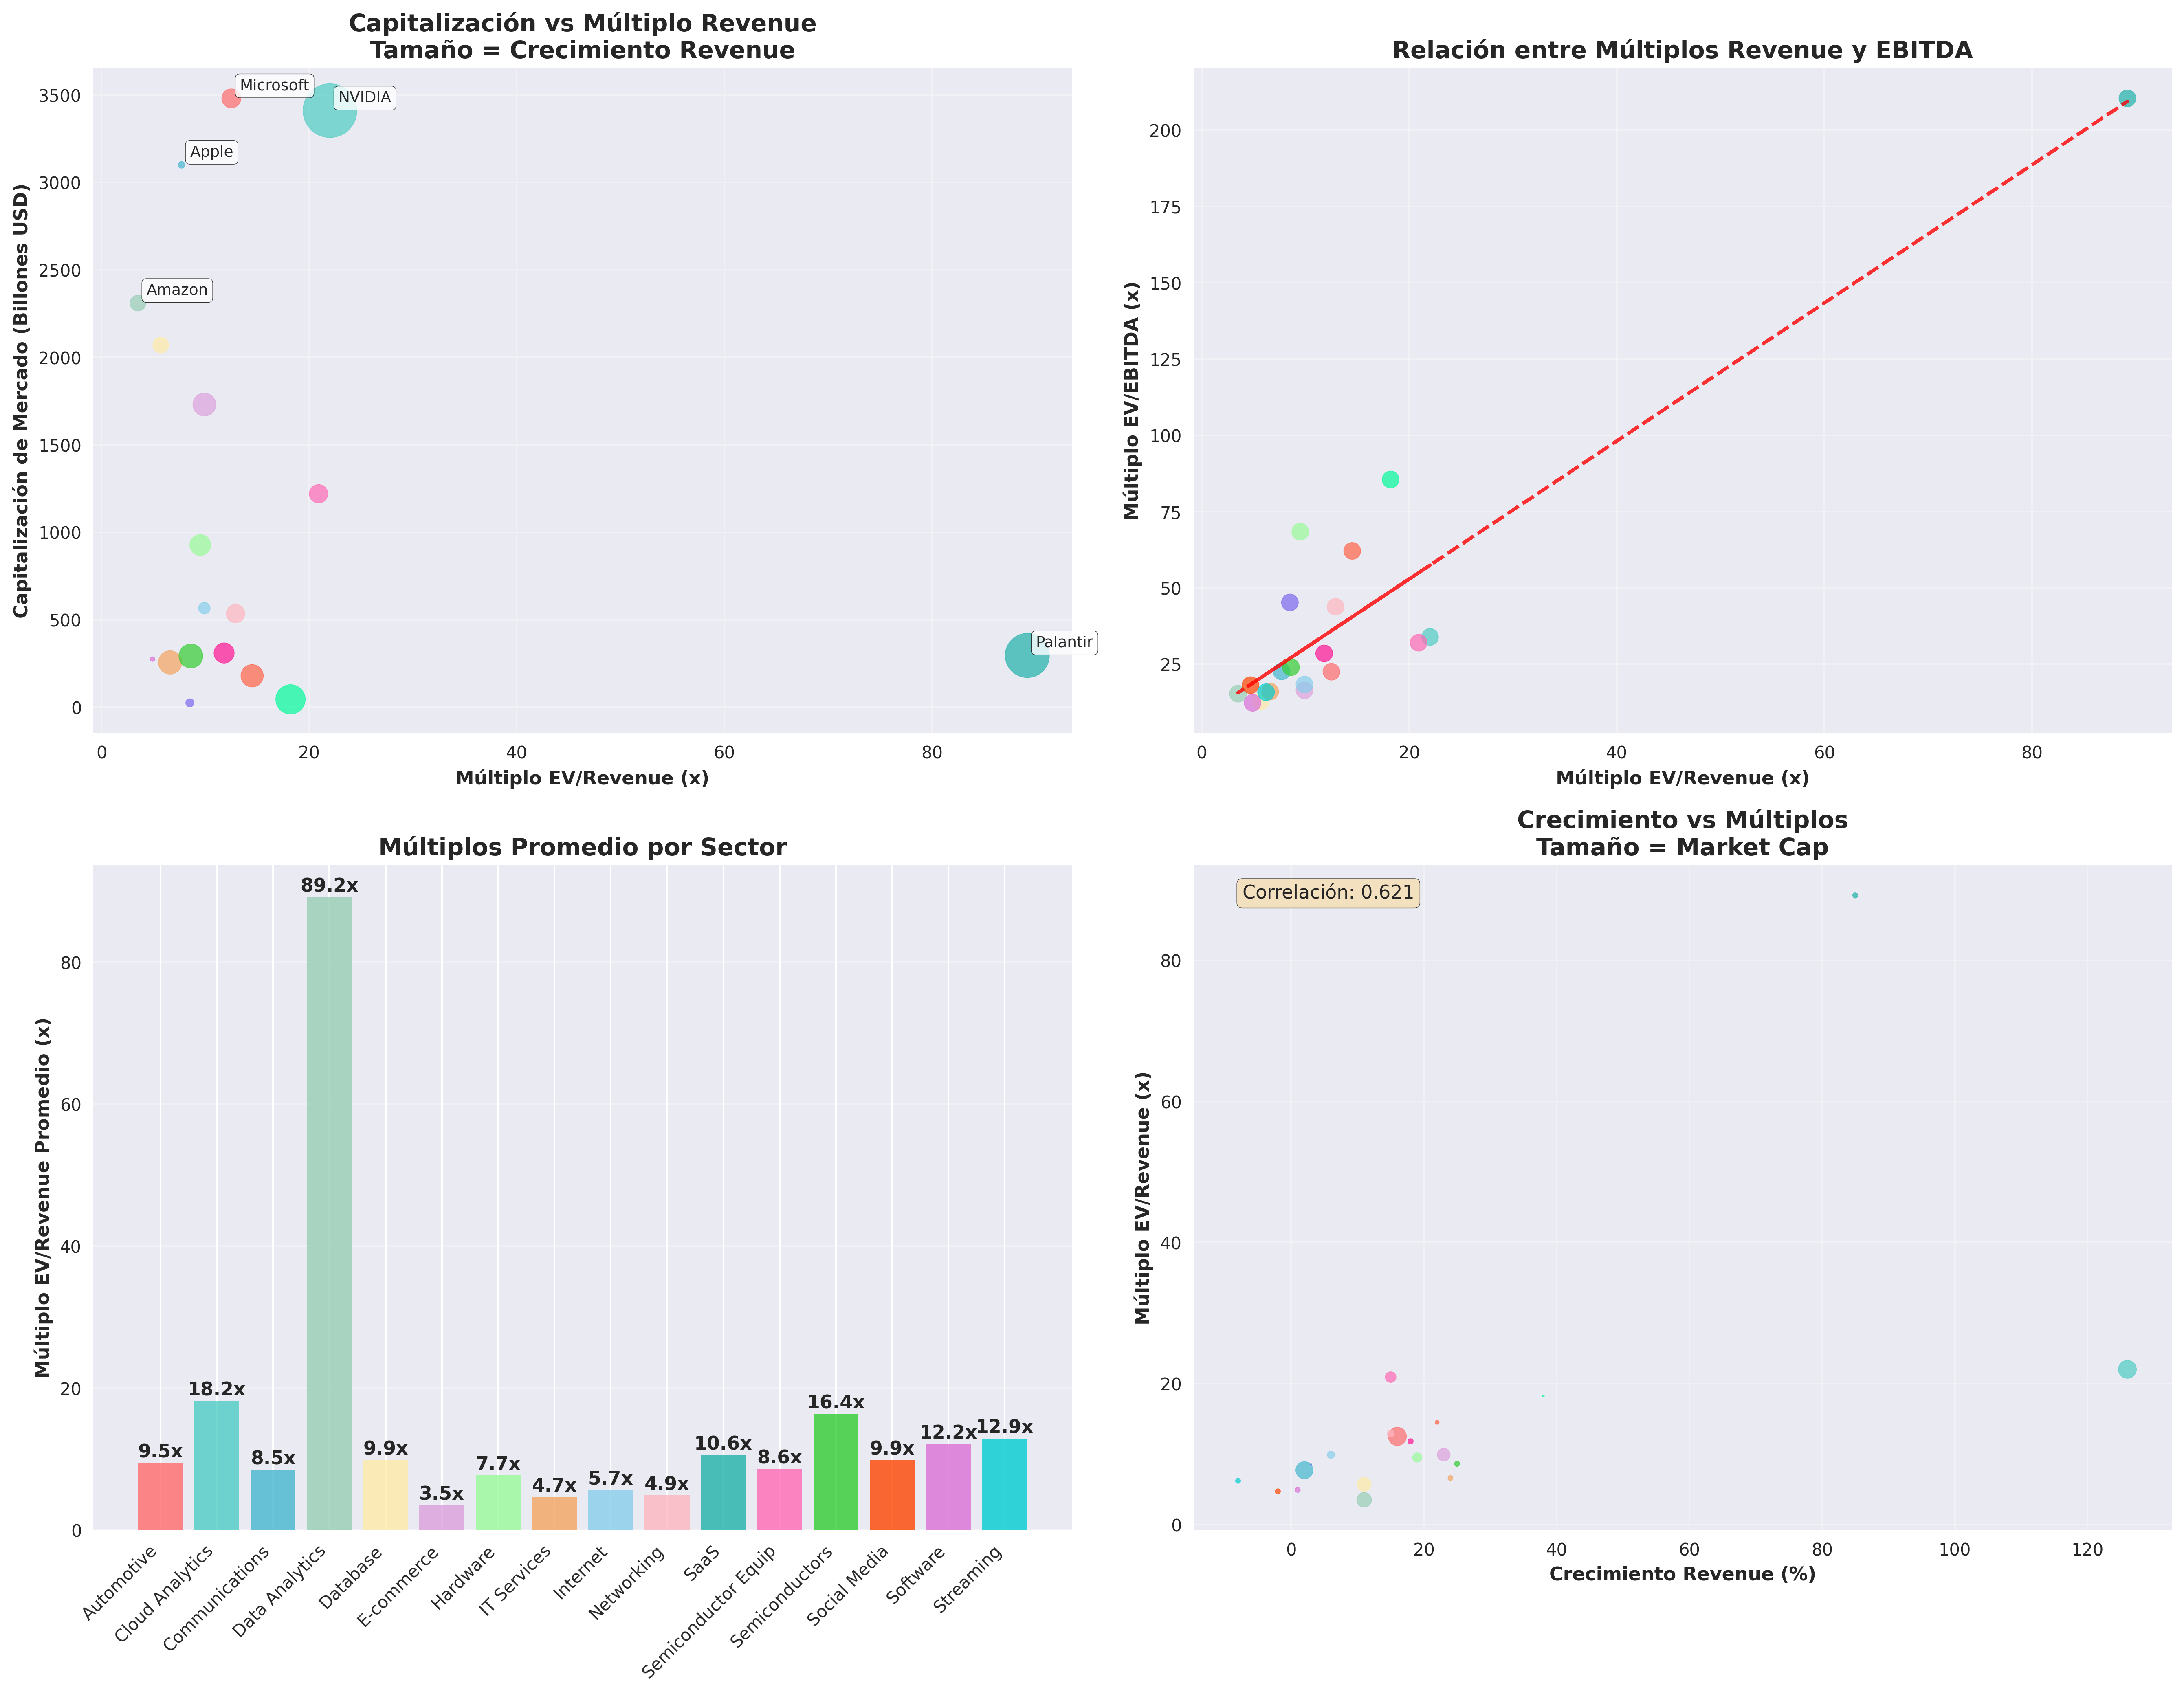
\includegraphics[width=0.9\textwidth]{figuras/analisis_empresas_lideres}
    \caption{Análisis comparativo de empresas tecnológicas líderes: capitalización de mercado, múltiplos de valoración y métricas de rentabilidad (2024)}
    \label{fig:comparacion_empresas}
\end{figure}

\begin{figure}[htbp]
    \centering
    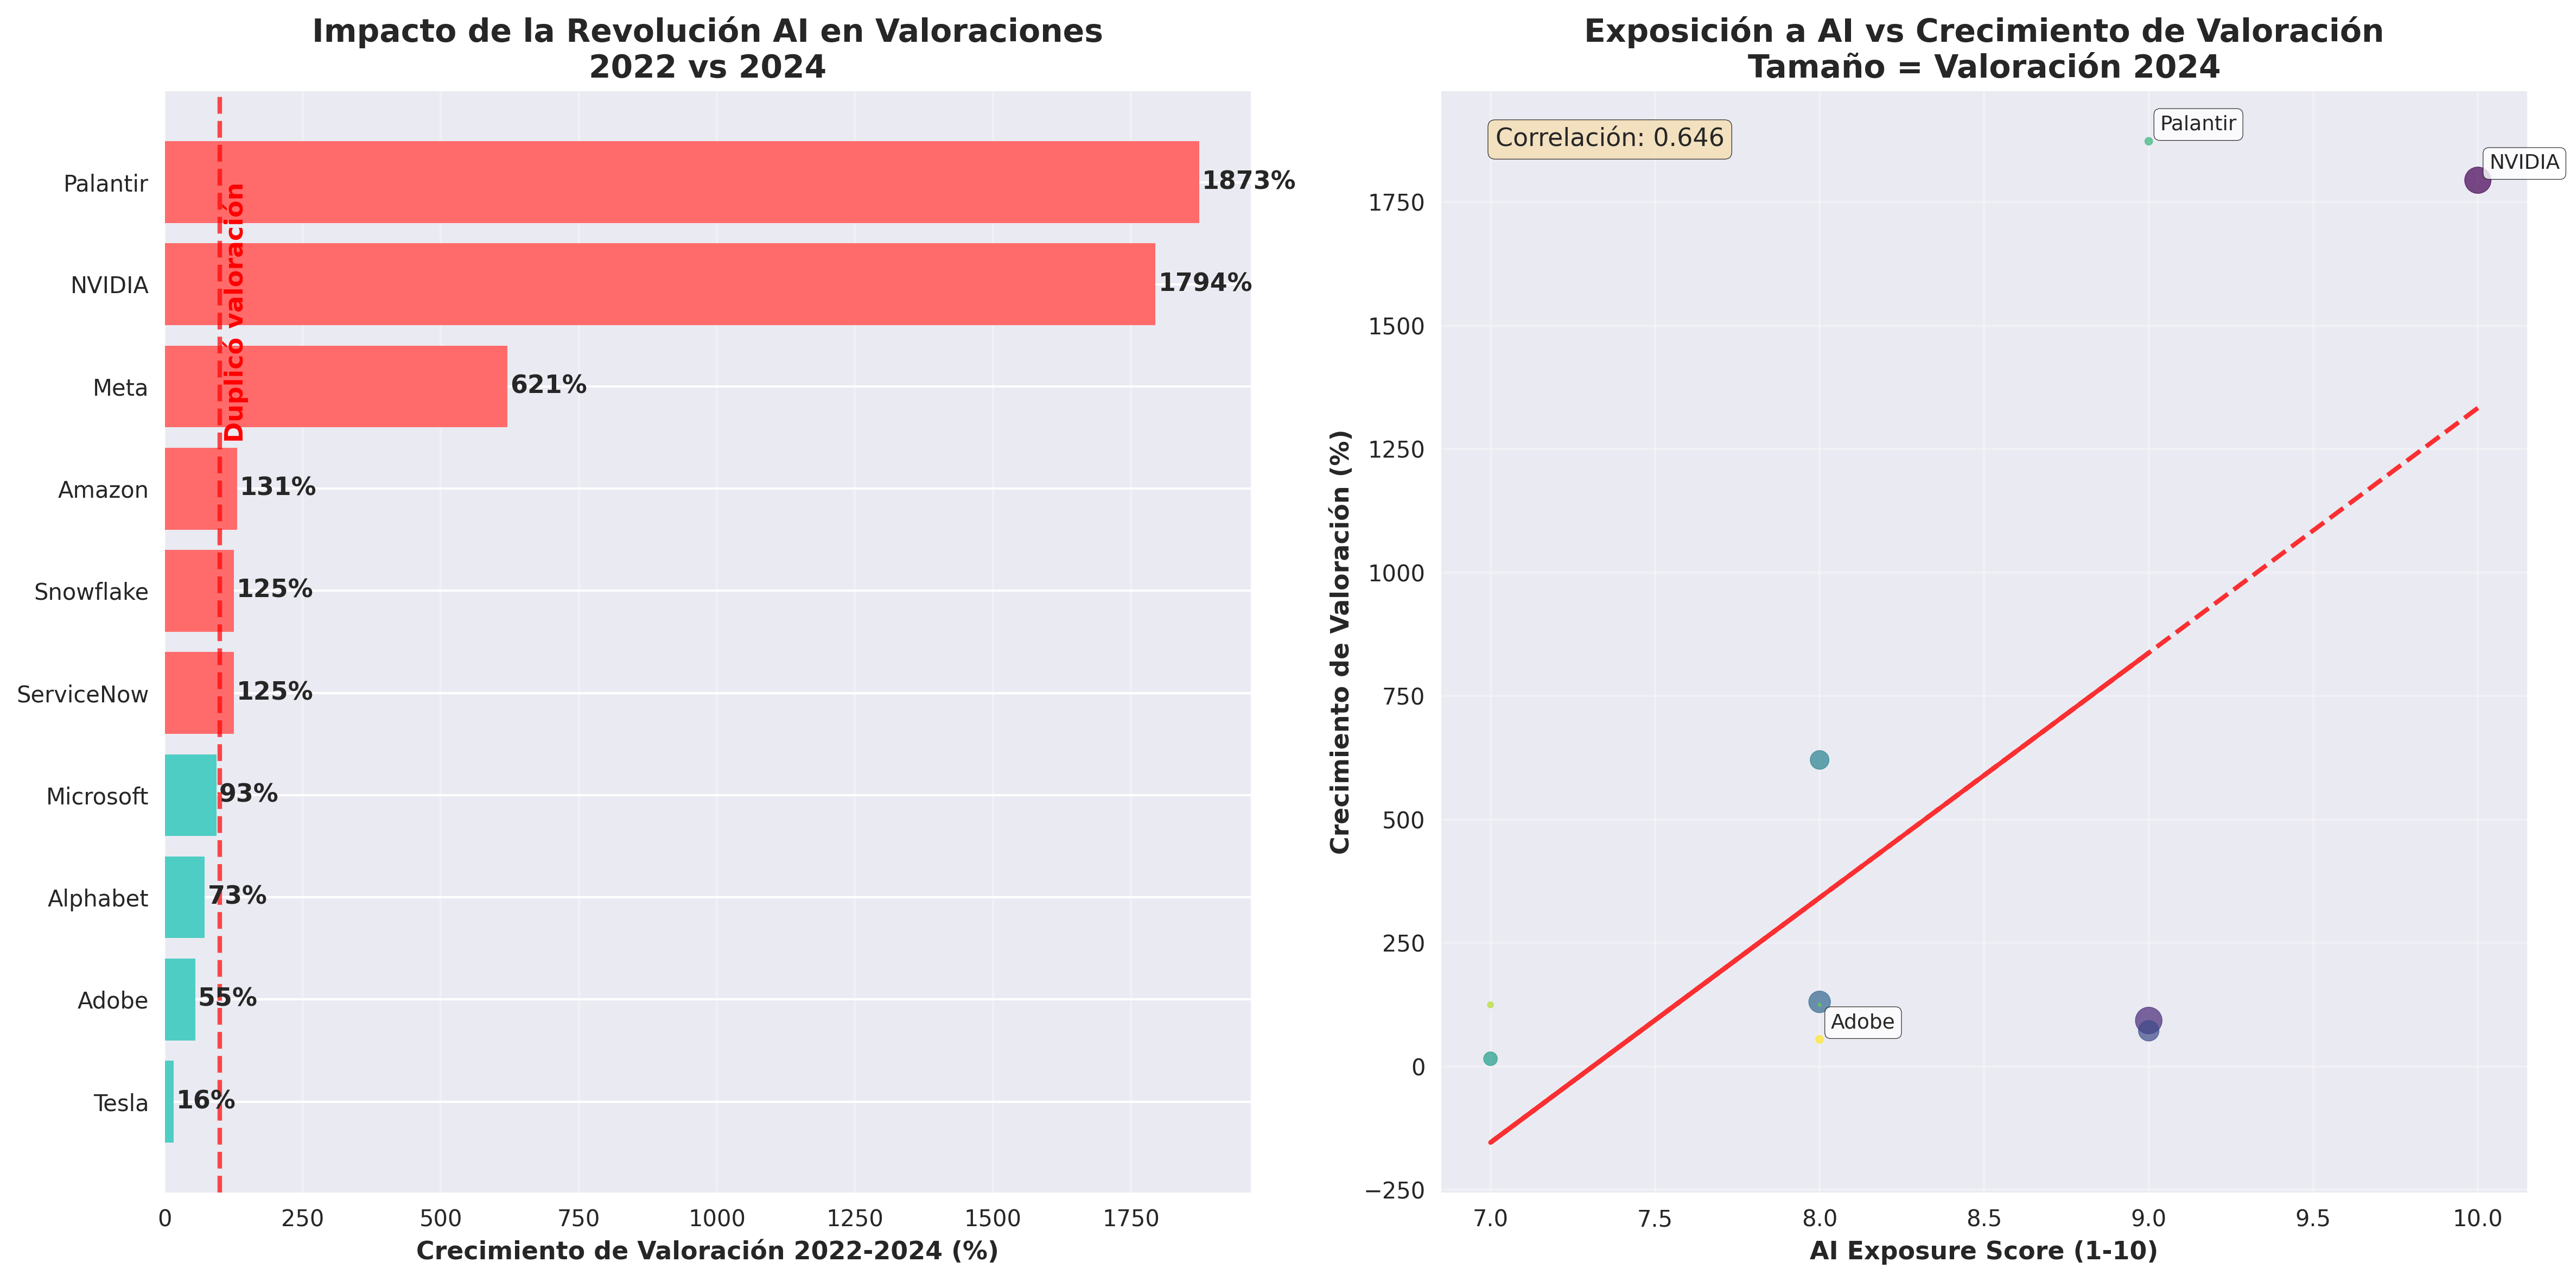
\includegraphics[width=0.9\textwidth]{figuras/impacto_ai_valoraciones}
    \caption{Impacto de la Inteligencia Artificial en valoraciones del sector tecnológico: crecimiento de capitalización y correlación con capacidades de IA (2022-2024)}
    \label{fig:impacto_ai}
\end{figure}

\subsection{Síntesis analítica de los casos}

Los casos estudiados ilustran lecciones fundamentales para la valoración de empresas tecnológicas que trascienden las particularidades individuales de cada empresa. Amazon demostró que el mercado puede respaldar estrategias de crecimiento a largo plazo cuando existe credibilidad demostrada en la capacidad de ejecución y una visión estratégica coherente respaldada por inversiones sustanciales en activos intangibles. Tesla ejemplificó cómo las narrativas de disrupción tecnológica pueden generar valoraciones que exceden considerablemente los fundamentos financieros actuales, reflejando expectativas especulativas sobre la materialización de mercados futuros y la monetización de opciones de crecimiento.

Google ilustró la importancia crítica de los activos intangibles superiores ---algoritmos, datos, efectos de red--- que pueden generar posiciones competitivas virtualmente dominantes y márgenes operativos excepcionales sostenibles a largo plazo. WeWork, por el contrario, subrayó que el mercado eventualmente exige coherencia entre la narrativa corporativa y la realidad operativa, y que las valoraciones basadas principalmente en expectativas sin fundamento empírico pueden colapsar dramáticamente cuando se exponen al escrutinio de inversionistas institucionales sofisticados.

El análisis contemporáneo de empresas en la era de la IA confirma que la diferenciación tecnológica real ---como la demostrada por NVIDIA en semiconductores especializados--- puede sostener múltiplos excepcionales cuando se combina con ejecución operativa sólida y barreras de entrada defendibles. Paralelamente, empresas como Palantir evidencian que el mercado continúa dispuesto a asignar valoraciones elevadas basadas en potencial futuro, aunque con niveles de riesgo proporcionalmente superiores reflejados en costos de capital más altos.

En síntesis, los casos analizados revelan que las empresas tecnológicas exitosas terminan validando sus valoraciones inicialmente elevadas a través de la materialización de crecimiento rentable sostenible y la demostración de ventajas competitivas duraderas, mientras que aquellas incapaces de demostrar viabilidad económica fundamental experimentan correcciones severas en sus valuaciones de mercado que pueden llegar hasta el colapso total del valor. 
\section{Tendencias actuales en la era digital}

La valuación de empresas tecnológicas evoluciona con las condiciones de mercado y los cambios en la percepción de inversionistas. En los últimos años se han observado tendencias clave que están moldeando los criterios de valuación en un contexto de mayor madurez y exigencia hacia el sector tecnológico. El año 2024 ha marcado un punto de inflexión significativo, caracterizado por la consolidación del financiamiento global de capital de riesgo en 314 mil millones de dólares ---un crecimiento del 3\% respecto a 2023--- pero con una concentración sin precedentes en el sector de Inteligencia Artificial \citep{pitchbook2024,carta2024}.

\subsection{Dominancia de intangibles y revolución de la Inteligencia Artificial}

A nivel agregado, los activos intangibles ---propiedad intelectual, capital de conocimiento, \emph{software}, datos, marca--- explican actualmente la mayor parte de la capitalización de las empresas líderes. Esta tendencia se ha acelerado dramáticamente, donde según datos actualizados de la Organización Mundial de la Propiedad Intelectual, los activos intangibles corporativos globales alcanzaron aproximadamente 80 billones de dólares en 2024, representando un crecimiento sustancial desde los 61.9 billones reportados en 2023 \citep{wipo2025}. En el contexto estadounidense, esta evolución es aún más pronunciada: las empresas mantienen una relación promedio del 90\% entre activos intangibles y valor empresarial, confirmando que los intangibles representan hasta el 90\% del valor del S\&P 500 \citep{oceantomo2024}.

El impacto de la Inteligencia Artificial ha redefinido fundamentalmente el panorama de valuación tecnológica durante 2024. Las empresas relacionadas con IA captaron el 48\% de toda la inversión de capital de riesgo global, superando los 100 mil millones de dólares en financiamiento ---un incremento del 80\% interanual--- \citep{pitchbook2024}. Este fenómeno trasciende la simple especulación: representa una reevaluación estructural de activos donde la capacidad de procesamiento de datos, algoritmos propietarios y infraestructura de aprendizaje automático se han convertido en los activos intangibles más valorados del mercado.

Esta evolución está impulsando una reevaluación fundamental de los estándares de contabilidad y valoración tradicionales, donde los organismos internacionales de regulación contable proponen mejoras sustanciales en la divulgación de información sobre activos intangibles, desarrollando nuevos marcos de reporte de capital intelectual y métricas de innovación que complementen los estados financieros tradicionales. Las empresas tecnológicas líderes como NVIDIA experimentaron valorizaciones extraordinarias durante 2024, convirtiéndose temporalmente en una de las cinco empresas más valiosas del mundo tras reportar demanda excepcional de sus chips especializados para IA, evidenciando cómo el mercado incorpora rápidamente la perspectiva de nuevos catalizadores de crecimiento basados en activos intangibles \citep{nvidia2024}.

En la práctica, los valuadores incorporan este cambio reconociendo que la brecha entre valor en libros y valor de mercado puede ser enorme y constituir una situación normal en empresas tecnológicas, reflejando activos reales no contabilizados más que una <<burbuja>> especulativa. Las fusiones y adquisiciones en el sector tecnológico frecuentemente implican pago de un \emph{goodwill} muy elevado, justificado precisamente por el valor de estos activos intangibles no registrados contablemente.

Tras un largo período de tasas de interés extremadamente bajas durante la década de 2010, a partir de 2022 las condiciones financieras cambiaron dramáticamente con aumentos significativos en las tasas de interés globales implementados para combatir la inflación. El costo de capital de las empresas tecnológicas experimentó incrementos significativos, generando un impacto notable en sus valoraciones donde el aumento en las tasas de descuento reduce matemáticamente el valor presente de los flujos de caja futuros, efecto particularmente pronunciado en empresas tecnológicas donde gran parte del valor reside en expectativas de flujos distantes. Durante 2022-2023, muchas acciones tecnológicas de alto crecimiento sufrieron caídas pronunciadas como resultado directo de esta revaluación.

Este cambio en las condiciones financieras se reflejó también en la actividad corporativa del sector tecnológico, donde el número de fusiones y adquisiciones experimentó una caída aproximada del 25\% interanual en la primera mitad de 2024, alcanzando mínimos de cuatro años y reflejando una menor disposición de los inversionistas a pagar múltiplos elevados en un entorno de capital considerablemente más costoso. Asimismo, 2022 marcó un enfriamiento drástico en las salidas a bolsa (IPOs) tecnológicas: el volumen de IPOs en Estados Unidos cayó 88\% respecto al año previo, tocando su nivel más bajo en 32 años. No obstante, durante 2024 se observan señales de recuperación selectiva en el mercado de salidas a bolsa, particularmente para empresas tecnológicas que demuestran métricas sólidas de rentabilidad y posicionamiento estratégico en sectores de alta demanda como la IA \citep{renaissance2024}.

\subsection{Transición hacia la disciplina financiera y nuevos múltiplos de valoración}

Durante la década de 2010, predominó entre empresas tecnológicas ---especialmente \emph{startups} apoyadas por capital de riesgo--- la filosofía del crecimiento acelerado incluso a costa de pérdidas operativas. Sin embargo, desde 2022 se percibe un cambio fundamental de enfoque hacia la rentabilidad y la eficiencia operativa, tendencia que se consolidó definitivamente durante 2024. Los datos actuales revelan una transformación dramática en los requisitos de financiamiento: las empresas Serie A ahora necesitan una mediana de 2.5 millones de dólares en ingresos anuales, un incremento del 75\% comparado con los niveles de 2021 \citep{carta2024}.

Los inversionistas activistas y fondos institucionales han intensificado la presión sobre las empresas tecnológicas para mejorar sus márgenes de beneficio, recortar gastos considerados innecesarios, y demostrar un camino claro y creíble hacia la generación de ganancias sustentables. Una encuesta de \cite{alixpartners2023} a ejecutivos tecnológicos reveló que en 2023 un 56\% ya priorizaba la rentabilidad igual o por encima del crecimiento, y que en los próximos dos años cerca del 74\% de las empresas tecnológicas planean enfocarse en rentabilidad sobre crecimiento.

Los múltiplos de valoración han experimentado una normalización significativa, particularmente evidente en el sector de \emph{Software as a Service} (SaaS). Las empresas SaaS públicas cotizan actualmente en un rango de 7.0x a 7.3x sus ingresos anuales, mientras que las empresas privadas del sector mantienen múltiplos de 4.8x a 5.3x ingresos durante 2024-2025 \citep{saasmetrics2024}. Esta normalización representa una estabilización después del declive significativo desde los picos históricos de 2021, cuando muchas empresas SaaS podían valorarse a 20x o más sus ingresos anuales.

Este giro estratégico se manifiesta en hechos concretos y medibles, donde las grandes empresas tecnológicas anunciaron despidos masivos y programas de reducción de gastos durante 2022-2023, mientras que las \emph{startups} han comenzado a enfatizar métricas de economía unitaria (\emph{unit economics}) por encima del simple crecimiento de usuarios. Paralelamente, las valoraciones en rondas de financiamiento tardías ahora favorecen claramente a empresas que demuestran capacidad de alcanzar el punto de equilibrio en flujo de caja (\emph{cash-flow breakeven}). En términos de valoración, esto implica que los múltiplos de ingresos se han contraído significativamente, mientras que los inversores vuelven a examinar múltiplos de ganancias o EBITDA con mayor atención.

La narrativa ha transitado de <<crece primero, ya monetizarás>> hacia <<muestra que puedes monetizar, aunque sacrifiques algo de crecimiento>>, valorándose ahora el concepto de crecimiento eficiente que combina expansión con disciplina operativa. Las empresas que demuestran capacidad de generar flujos de caja libres positivos o un camino claro hacia la rentabilidad reciben valoraciones premium, mientras que aquellas que no logran articular economías unitarias sólidas experimentan descuentos significativos en sus valoraciones.

Los años 2020-2021, impulsados por liquidez abundante, tasas cero y optimismo en la digitalización derivado de la pandemia, presenciaron valoraciones récord en tecnológicas públicas y privadas. Durante este período, el índice Nasdaq alcanzó máximos históricos sin precedentes, mientras que solo en el primer semestre de 2021 se invirtieron más de \$300.000 millones en capital de riesgo a nivel mundial. Esta euforia generalizada condujo a valoraciones posiblemente excesivas, caracterizadas por una expansión significativa de múltiplos que reflejaba expectativas optimistas extremas sobre el crecimiento futuro del sector.

A partir de finales de 2021 y durante 2022, se produjo una corrección generalizada en las valoraciones tecnológicas donde muchas acciones del sector experimentaron caídas del 50\% o superiores desde sus máximos históricos, mientras que el financiamiento privado también se contrajo significativamente. La corrección ha resultado en una realidad donde aproximadamente el 50\% de las empresas unicornio posiblemente ya no merecen valoraciones superiores a mil millones de dólares según criterios actuales de mercado, con el 30\% de ellas efectivamente valuadas por debajo de ese umbral según estimaciones de valor justo de mercado \citep{silicon2024}.

Sin embargo, la corrección no afectó uniformemente a todas las empresas: aquellas de mayor calidad o con flujos de caja robustos resistieron mejor, indicando una vuelta a la racionalidad en los criterios de valuación donde los inversores discriminan más según la posición competitiva real y la evidencia de rentabilidad. Por ejemplo, empresas de \emph{software} empresarial con suscripciones y flujos predecibles mantuvieron múltiplos relativamente altos, mientras que \emph{fintechs} o \emph{marketplaces} que no lograron demostrar economía unitaria sólida vieron sus valoraciones reducidas drásticamente.

\subsection{Nuevas fronteras tecnológicas y consideraciones ESG}

La era digital continúa presentando olas de innovación tecnológica ---\emph{blockchain} y criptomonedas, metaverso, y más recientemente la explosión de la Inteligencia Artificial generativa--- que influyen significativamente en las valoraciones del sector. El año 2024 ha sido definido como el año de la IA, donde compañías vinculadas a esta tecnología experimentaron aumentos pronunciados en sus precios ante la expectativa de que la IA revolucionará múltiples industrias. NVIDIA, proveedor de GPUs para IA, se convirtió temporalmente en una de las 5 empresas más valiosas del mundo tras reportar demanda excepcional de sus chips, evidenciando cómo el mercado incorpora rápidamente la perspectiva de nuevos catalizadores de crecimiento.

Patrones similares se observaron durante la fiebre del metaverso en 2021 y el auge de las criptomonedas y NFT en sus respectivos momentos de máxima popularidad, aunque muchas de esas expectativas posteriormente se desinflaron parcialmente al enfrentarse a los retos de implementación real. La lección fundamental es que las tendencias tecnológicas emergentes pueden alterar criterios de valuación en el corto plazo, frecuentemente descontando muchos años de crecimiento futuro por adelantado. Los analistas deben reconocer el potencial disruptivo de estas tecnologías mientras mantienen prudencia para no sobreestimar impactos inmediatos que podrían no materializarse según las expectativas iniciales.

Aunque no constituye un factor exclusivamente digital, en los últimos años los inversionistas prestan atención creciente a temas de sostenibilidad, gobierno corporativo y responsabilidad social (ESG, por sus siglas en inglés). Las empresas tecnológicas que demuestran sólido desempeño en criterios ESG pueden atraer una base de inversores más amplia y paciente, lo cual tiende a favorecer sus valoraciones mediante la reducción del costo de capital aplicable. Por el contrario, cuestiones como violaciones a la privacidad de datos, prácticas consideradas monopólicas o impacto social negativo de la tecnología pueden restar valor si generan escrutinio regulatorio o riesgos reputacionales significativos.

La evaluación cualitativa contemporánea incorpora también una perspectiva ESG donde un modelo de negocio percibido como predatorio o no ético puede recibir múltiplos más bajos o verse penalizado por desinversiones de fondos con criterios de sostenibilidad. Esta tendencia refleja una evolución en los criterios de inversión hacia consideraciones que trascienden los retornos financieros inmediatos, incorporando el impacto a largo plazo de las prácticas empresariales en la sociedad y el medio ambiente.

En síntesis, las tendencias actuales reflejan un entorno de mayor madurez y exigencia en la valuación de empresas tecnológicas, donde la disciplina financiera ha emergido como prioridad tras años de expansiones exuberantes. Las tasas de interés más elevadas exigen resultados más concretos y demostrables, mientras que el foco en rentabilidad ha llevado a los inversionistas a demandar beneficios actuales o al menos un camino claro hacia su materialización. El concepto de crecimiento eficiente ha ganado prominencia, premiando la capacidad de combinar expansión con disciplina operativa. La revolución de la Inteligencia Artificial ha introducido nuevos paradigmas de valoración de activos intangibles, mientras que la normalización de múltiplos refleja un retorno hacia criterios de valuación más fundamentados en métricas financieras tradicionales. Sin embargo, la innovación continúa impulsando nuevas expectativas y oportunidades de valor, requiriendo que las valoraciones combinen análisis de datos duros con evaluación informada sobre desarrollos futuros, manteniendo un balance apropiado para evitar tanto la euforia injustificada como el escepticismo excesivo.  
\chapter{Conclusiones}

La valuación de empresas tecnológicas es un campo fascinante y complejo, donde confluyen los principios financieros tradicionales con las particularidades de la nueva economía digital. A lo largo de esta investigación se han revisado los fundamentos teóricos de la valoración corporativa y se ha analizado cómo aplicarlos al contexto de las empresas de tecnología, incorporando las adaptaciones necesarias.

\section{Principales hallazgos}

La presente investigación ha permitido identificar elementos fundamentales que caracterizan la valoración de empresas tecnológicas y que constituyen aportes significativos al conocimiento en este campo especializado.

Los fundamentos financieros tradicionales mantienen su vigencia teórica, siendo el concepto central del valor presente de flujos de caja futuros la piedra angular conceptual de la valoración empresarial. El método de descuento de flujos de fondos (\emph{DCF}) continúa proporcionando el marco analítico más sólido para la estimación del valor intrínseco. Sin embargo, las empresas tecnológicas obligan a extender significativamente este marco hacia horizontes temporales más largos y escenarios de mayor incertidumbre, dado que gran parte de su valor económico radica en flujos esperados a muy largo plazo y sujetos a riesgos específicos del sector. En este contexto, herramientas metodológicas complementarias como las opciones reales cobran particular relevancia al formalizar el valor de la flexibilidad estratégica y las oportunidades de crecimiento, aspectos especialmente relevantes en compañías de base tecnológica.

La complejidad inherente a la valoración tecnológica demanda necesariamente una visión metodológica integral. Ningún método único puede capturar completamente la realidad multifacética de las empresas \emph{tech}, obligando a los analistas a combinar diversos enfoques: el \emph{DCF} multi-etapas para valorar la trayectoria temporal de flujos, los múltiplos de mercado para reflejar las condiciones sectoriales actuales, los métodos patrimoniales cuando resultan aplicables, y los enfoques específicos orientados a la lógica de inversionistas especializados como el \emph{venture capital method}. El contraste sistemático de resultados obtenidos mediante diferentes metodologías aumenta significativamente la robustez de la valoración y permite identificar supuestos inconsistentes, aspecto particularmente crítico en empresas tecnológicas donde estas discrepancias emergen frecuentemente y deben explicarse mediante los factores particulares de cada caso específico.

Las empresas tecnológicas exhiben características distintivas que inciden tanto cuantitativa como cualitativamente en su proceso de valoración. Estas organizaciones presentan rasgos diferenciadores ---predominio de activos intangibles, modelos de negocio altamente escalables, ciclos de vida dinámicos--- que requieren adaptaciones metodológicas específicas. La mayor parte del valor económico de las empresas \emph{tech} suele residir en activos intangibles y en el potencial de crecimiento futuro, más que en activos tangibles actuales o en la rentabilidad presente, justificando múltiplos aparentemente elevados donde el mercado capitaliza no los beneficios actuales sino las posibilidades de generación de valor futuro. No obstante, estos intangibles y expectativas de crecimiento también implican riesgos significativos, ya que no todas las empresas lograrán materializar sus expectativas iniciales, requiriendo que la valoración incorpore explícitamente primas de riesgo superiores y análisis de escenarios alternativos.

La valoración efectiva de empresas tecnológicas demanda la integración sistemática de factores cuantitativos y cualitativos. En el sector tecnológico, más que en cualquier otro ámbito empresarial, los elementos cualitativos ---visión estratégica, capacidad de innovación, calidad del talento humano, fortaleza de marca, presencia de efectos de red--- moldean directamente los resultados cuantitativos expresados en tasas de crecimiento, márgenes operativos y generación de flujos de caja. Un producto superior respaldado por un modelo de negocio sólido y un equipo directivo excelente probablemente se traducirá en métricas financieras robustas a lo largo del tiempo, mientras que debilidades cualitativas fundamentales tarde o temprano erosionarán los resultados numéricos. Esta interrelación obliga al evaluador a incorporar ambas dimensiones analíticas de manera integrada, donde la valoración efectiva de una empresa \emph{tech} combina necesariamente el rigor analítico cuantitativo con una comprensión estratégica profunda del negocio y su contexto competitivo.

\section{Lecciones de los casos estudiados}

Los casos estudiados (Amazon, Tesla, Google, \emph{WeWork}, entre otros) ilustran en vivo las oportunidades y trampas de la valoración en tecnología:

\begin{itemize}
    \item \textbf{Amazon}: Aprendimos cómo el mercado puede apoyar estrategias de largo plazo y valorar intangibles incluso en ausencia de utilidades inmediatas
    \item \textbf{Tesla}: Mostró cómo las narrativas de disrupción pueden inflar valoraciones muy por encima de fundamentos actuales
    \item \textbf{Google}: Ejemplificó la importancia de un activo intangible superior que genera dominancia casi natural del mercado
    \item \textbf{\emph{WeWork}}: subrayó que el mercado eventualmente exige resultados
\end{itemize}

En general, \textbf{los casos muestran que las empresas tecnológicas que triunfan terminan validando sus valoraciones altas a través de crecimiento rentable, mientras que las que fallan ven sus valoraciones corregirse drásticamente}.

\section{El nuevo paradigma de valoración}

\textbf{Tendencias actuales: prudencia y nueva normalidad}: tras la revisión de tendencias, se concluye que estamos en una fase en la que la valoración de empresas tecnológicas se ha vuelto más exigente y selectiva en comparación con algunos años recientes.

\textbf{El entorno de tasas de interés altas y capital más caro impone disciplina}: ya no es tan fácil justificar múltiplos indefinidamente expansivos sin demostración de rentabilidad en el horizonte. Las empresas \emph{tech} han tenido que adaptarse reduciendo costos y mostrando responsabilidad fiscal.

Los inversionistas han recalibrado sus modelos: hoy se valoran modelos de crecimiento eficiente y se hacen más diferenciaciones entre ganadores y perdedores en cada nicho.

Sin embargo, la innovación continua, y cuando surgen nuevas olas tecnológicas (\emph{IA}, etc.), el mercado reacciona incorporando esas expectativas. \textbf{El equilibrio entre visión de futuro y realismo presente será la piedra de toque de las valoraciones en adelante}.

\section{Reflexiones finales}

La valuación de empresas tecnológicas constituye un campo de conocimiento que demanda la combinación de fundamentos financieros sólidos con una comprensión profunda de las dinámicas específicas del sector tecnológico. Si bien supone enfrentar niveles elevados de incertidumbre y la complejidad inherente a la valoración de activos intangibles, la aplicación apropiada de herramientas metodológicas especializadas permite estimar rangos de valor económicamente razonables y profesionalmente defendibles.

El conjunto de herramientas fundamentales incluye el análisis \emph{DCF} multi-escenario como base conceptual, la valoración por opciones reales para capturar la flexibilidad estratégica, el análisis riguroso de comparables sectoriales, y la incorporación sistemática del juicio cualitativo informado. La efectividad del proceso de valoración depende críticamente de mantenerse actualizado con las tendencias evolutivas del sector, aplicar flexibilidad metodológica según las características específicas de cada empresa, y preservar la perspectiva fundamental de que detrás de cada proyección numérica subyacen supuestos sobre personas, productos, mercados y tecnologías.

La valoración efectiva de empresas tecnológicas requiere un enfoque intelectualmente riguroso pero metodológicamente creativo, capaz de captar tanto el valor tangible presente como el potencial latente de organizaciones que están redefiniendo continuamente los paradigmas de creación de valor en la economía digital contemporánea.

Para los profesionales especializados en valuación que trabajan con empresas tecnológicas, esta investigación sugiere la adopción de una perspectiva metodológica múltiple que evite la dependencia exclusiva de un solo enfoque de valoración, la inversión significativa de tiempo en comprender profundamente las características específicas del modelo de negocio evaluado, el uso sistemático de análisis de escenarios múltiples dada la alta incertidumbre inherente al sector, el mantenimiento de actualización continua ante la rápida evolución de tendencias tecnológicas y de mercado, y el equilibrio cuidadoso entre el reconocimiento del potencial de crecimiento y la evaluación realista de los riesgos asociados.

En un contexto económico donde los activos intangibles dominan progresivamente la creación de valor empresarial, la capacidad de valorar apropiadamente las empresas tecnológicas se convierte en una competencia profesional fundamental e ineludible para cualquier especialista en finanzas corporativas que aspire a mantenerse relevante en el panorama profesional contemporáneo. 

% Bibliografía
\cleardoublepage
\printbibliography[title=Bibliografía]

% Anexos (si los hay)
% \appendix
% \input{secciones/anexos}

\end{document} 